\section{Qualitative Possibilistic MDPs}
This section presents the uncertainty framework studied in this thesis:
namely, the model $\pi$-POMDP.
First of all, the Possibility Theory is presented, 
with a particular emphasis on the qualitative part 
of the theory. Qualitative conditioning is then presented,
as well as notions of independence.
Finally, the qualitative possibilistic counterpart of the MDPs 
called \textit{Qualitative Possibilistic MDPs}, or $\pi$-MDPs
are defined, followed by the \textit{Qualitative Possibilistic POMDPs}, or $\pi$-POMDPs.
\subsection{Possibility Theory}
\label{posspres}
The ``fuzzy sets'' introduced by Lotfi Zadeh \cite{Zadeh1965338}, 
have been studied by Didier Dubois \cite{didiersgroundhogday} and Henri Prade
and their contributions have led to the foundation of Possibility Theory \cite{DuPr1988.4}.

As in Probability Theory, this theory is based on the definition of an uncertainty measure,
called \textit{possibility measure}.
Unlike the probability measure $\mathbb{P}$ 
which is a classical measure (Definition \ref{measure}),
the \textit{possibility measure}, denoted by $\Pi$, is a \textit{fuzzy measure}, or \textit{capacity}.
For simplicity, a fuzzy measure is not supposed to be additive,
but just \textit{monotone}, as highlighted by Definition \ref{fuzzy_measure}.
In this thesis, Possibility Theory will only concern 
finite sets such as $\mathcal{S}$ and $\mathcal{O}$,
that is why definitions only concern finite sets.
\begin{Def}[Measure]
\label{measure}
A classical measure $\mathbb{M}$ on the finite set $\Omega$ is a function from $2^{\Omega}$ to $\mathbb{R}^{+}$ such that
\begin{itemize}
\item $\mathbb{M}(\emptyset) = 0$ (\textit{null empty set});
\item $\forall A,B \subseteq \Omega$ such that $A \cap B = \emptyset$, $\mathbb{M}(A \cup B ) = \mathbb{M}(A) + \mathbb{M}( B ) $ (\textit{additivity}).
\end{itemize}
\end{Def}

\begin{Def}[Fuzzy Measure]
\label{fuzzy_measure}
A fuzzy measure $\textgoth{M}$ on the finite set $\Omega$ is a function from $2^{\Omega}$ to $\mathbb{R}^{+}$ such that
\begin{itemize}
\item $\textgoth{M}(\emptyset) = 0$ (\textit{null empty set});
\item $\forall A,B \subseteq \Omega$ such that $A \subseteq B$, $\textgoth{M}(A) \leqslant \textgoth{M}(B)$ (\textit{monotonicity}).
\end{itemize}
\end{Def}
Note that a classical measure is a particular case of fuzzy measure
since classical measures are monotone: 
if $A \subset B$, 
\[ \mathbb{M}(B) = \mathbb{M} \paren{ (A \cap B) \cup (\overline{A} \cap B) } = \mathbb{M}( A ) + \mathbb{M} (\overline{A} \cap B) \geqslant  \mathbb{M}( A ), \]
where $\overline{A}$ is the complementary set of $A$ in $\Omega$ \textit{i.e.} $\overline{A} \cap A = \emptyset$, and $\overline{A} \cup A = \Omega$.

A possibility measure is also a particular case of fuzzy measure:
\begin{Def}[Possibility Measure]
\label{poss_measure}
A possibility measure on the finite set $\Omega$ is a fuzzy measure such that
\begin{itemize}
\item $\Pi(\Omega) = 1$ (\textit{normalization});
\item $\forall A,B \subset \Omega$, $\Pi \set{ A \cup B } = \max \big\{ \Pi(A), \Pi(B) \big\}$ (\textit{maxitivity}).
\end{itemize}
\end{Def}

Probability Theory models the uncertainty due to the variability of events:
in practice, used probabilities are estimated frequencies of events
stated as the actual variability model of events. 
Another view of this theory is De Finetti's one \cite{de1974theory}:
the probability value of an event is an exchangeable bet, \textit{i.e.}
the value in $[0,1]$ that a given person is willing to give
for the bet winning $1$ if the event is true.
However this person takes into account in her/his choice of value
that the bet can be reversed just before verifying if the event if true.
Indeed, she/he may be asked to get the chosen value,
and to give $1$ if the event is true.
As the probability values depend on a natural person,
who wants to guess the actual probability distribution 
as well as possible with respect to all her/his information about the event,
they are called \textit{subjective probabilities}:
that is why the theory based on this definition is called
Subjective Probability Theory.

Possibility Theory is devoted to uncertainty due to a lack of knowledge
or imprecision about an event.
Quantitative Possibility Theory can be seen as a special case of imprecise probabilities
\textit{i.e.} a possibility measure $\Pi$ represents a set of probability measures defined on $\Omega$,
denoted by $\mathcal{P}^{\Pi}$, and
each probability measure $\mathbb{P} \in \mathcal{P}^{\Pi}$ 
is a guess about the actual probabilistic model. 
The set $\mathcal{P}^{\Pi}$
is the set of each probability measure $\mathbb{P}$
such that $\forall A \subset \Omega$, $\mathbb{P}(A) \leqslant \Pi(A)$.
In this case, possibility measures are thus ``inflated'' probability measures,
in order to model that frequencies are not well known,
as illustrated by Figure \ref{figure_quantitativeposs}.
The possibility measure is then $\forall A \subset \Omega$, $\Pi(A) = \max_{\mathbb{P} \in \mathcal{P}^{\Pi}} \mathbb{P}(A)$.

If the set of probability distributions consists of 
all the probability distributions defined on $\Omega$,
\textit{i.e.} the probabilistic model is completely unknown,
and then $\forall A \subset \Omega$,
$\Pi(A) = \max_{\mathbb{P} \in \mathcal{P}^{\Pi}} \mathbb{P}(A) = 1$:
the ignorant possibility measure is equal to $1$ for each set $A \subset \Omega$,
a illustrated Figure \ref{poss1}.
On the contrary, if the actual elementary event is known to be $\omega_A$,
$\forall \omega \in \Omega$ such that $\omega \neq \omega_A$, $\Pi \paren{ \set{\omega} } = \mathbb{P} \paren{ \set{\omega} } = 0$
and  $\Pi \paren{ \set{\omega_A} } = \mathbb{P} \paren{ \set{\omega_A} } = 1$,
as illustrated Figure \ref{poss4}.
It is worth noting that there exists some sets of probability distributions
which are not represented by any quantitative possibility distribution:
for instance, the set of probability distributions on $\Omega = \set{\omega_A,\omega_B}$,
$\set{ \mathbb{P} \sachant \mathbb{P}(\omega_A) \geqslant 0.1, \mathbb{P}(\omega_B) \geqslant 0.1  }$.

\begin{figure}
\begin{subfigure}{0.245\linewidth}
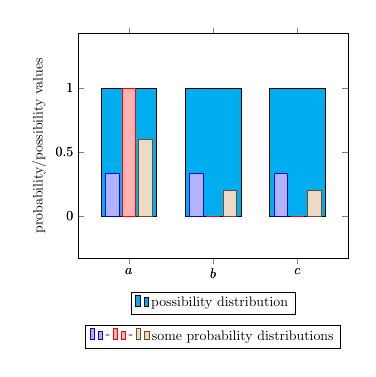
\begin{tikzpicture}[scale=0.5]
\begin{axis}[ymax=1.1, ymin=0, ybar, enlargelimits=0.3, legend style={at={(0.5,-0.15)}, anchor=north}, ylabel={probability/possibility values}, symbolic x coords={$a$, $b$, $c$}, xtick=data, bar width=40pt] 
\addplot [fill=cyan] coordinates {($a$,1) ($b$,1) ($c$,1)}; 
\legend{possibility distribution}
\end{axis}
\begin{axis}[ymax=1.1, ybar, enlargelimits=0.3, legend style={at={(0.5,-0.3)}, anchor=north, legend columns=-1}, ylabel={\hspace{1cm}}, symbolic x coords={$a$, $b$, $c$}, xtick=data,] 
\addplot coordinates {($a$,0.333) ($b$,0.333) ($c$,0.333)}; 
\addplot coordinates {($a$,1) ($b$,0) ($c$,0)}; 
\addplot coordinates {($a$,0.6) ($b$,0.2) ($c$,0.2)}; 
\legend{-,-,some probability distributions}
\end{axis} 
\end{tikzpicture}
\caption{ignorant distribution}
\label{poss1}
\end{subfigure}
\hspace{-0.15cm}
\begin{subfigure}{0.245\linewidth}
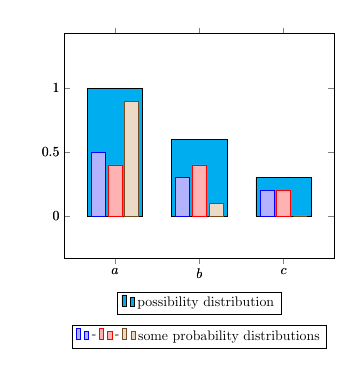
\begin{tikzpicture}[scale=0.5]
\begin{axis}[ymax=1.1, ymin=0, ybar, enlargelimits=0.3, legend style={at={(0.5,-0.15)}, anchor=north}, ylabel={\hspace{1cm}}, symbolic x coords={$a$, $b$, $c$}, xtick=data, bar width=40pt] 
\addplot [fill=cyan] coordinates {($a$,1) ($b$,0.6) ($c$,0.3)}; 
\legend{possibility distribution} 
\end{axis}
\begin{axis}[ymax=1.1, ymin=0, ybar, enlargelimits=0.3, legend style={at={(0.5,-0.3)}, anchor=north, legend columns=-1}, ylabel={\hspace{1cm}}, symbolic x coords={$a$, $b$, $c$}, xtick=data,] 
\addplot coordinates {($a$,0.5) ($b$,0.3) ($c$,0.2)}; 
\addplot coordinates {($a$,0.4) ($b$,0.4) ($c$,0.2)}; 
\addplot coordinates {($a$,0.9) ($b$,0.1) ($c$,0)}; 
\legend{-,-,some probability distributions}
\end{axis} 
\end{tikzpicture}
\caption{three different degrees}
\label{poss2}
\end{subfigure}
\hspace{-0.25cm}
\begin{subfigure}{0.245\linewidth}
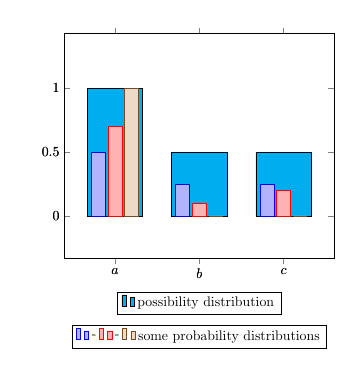
\begin{tikzpicture}[scale=0.5]
\begin{axis}[ymax=1.1, ymin=0, ybar, enlargelimits=0.3, legend style={at={(0.5,-0.15)}, anchor=north}, ylabel={\hspace{1cm}}, symbolic x coords={$a$, $b$, $c$}, xtick=data, bar width=40pt] 
\addplot [fill=cyan] coordinates {($a$,1) ($b$,0.5) ($c$,0.5)}; 
\legend{possibility distribution} 
\end{axis}
\begin{axis}[ymax=1.1, ybar, enlargelimits=0.3, legend style={at={(0.5,-0.3)}, anchor=north, legend columns=-1}, ylabel={\hspace{1cm}}, symbolic x coords={$a$, $b$, $c$}, xtick=data,] 
\addplot coordinates {($a$,0.5) ($b$,0.25) ($c$,0.25)}; 
\addplot coordinates {($a$,0.7) ($b$,0.1) ($c$,0.2)}; 
\addplot coordinates {($a$,1) ($b$,0) ($c$,0)}; 
\legend{-,-,some probability distributions}
\end{axis} 
\end{tikzpicture}
\caption{two different degrees}
\label{poss3}
\end{subfigure}
\hspace{-0.25cm}
\begin{subfigure}{0.245\linewidth}
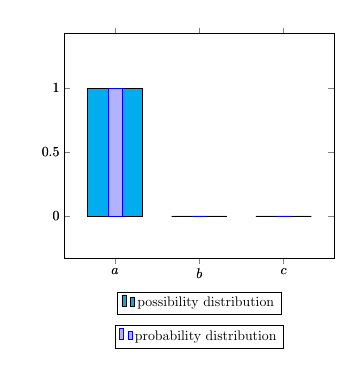
\begin{tikzpicture}[scale=0.5]
\begin{axis}[ymax=1.1, ymin=0, ybar, enlargelimits=0.3, legend style={at={(0.5,-0.15)}, anchor=north}, ylabel={\hspace{1cm}}, symbolic x coords={$a$, $b$, $c$}, xtick=data, bar width=40pt] 
\addplot [fill=cyan] coordinates {($a$,1) ($b$,0) ($c$,0)}; 
\legend{possibility distribution} 
\end{axis}
\begin{axis}[ymax=1.1, ybar, enlargelimits=0.3, legend style={at={(0.5,-0.3)}, anchor=north, legend columns=-1}, ylabel={\hspace{1cm}}, symbolic x coords={$a$, $b$, $c$}, xtick=data,] 
\addplot coordinates {($a$,1) ($b$,0) ($c$,0)}; 
\legend{probability distribution}
\end{axis} 
\end{tikzpicture}
\caption{determinism}
\label{poss4}
\end{subfigure}
\caption[Quantitative possibility distributions and associated probability distributions]{Example of quantitative possibility distributions (thick blue), and some of the associated probability distributions (thin) 
\textit{i.e.} some of the probability measures encoded by the possibility distribution. Distributions are defined on $\Omega = \set{a,b,c}$.}
\label{figure_quantitativeposs}
\end{figure}

Unlike quantitative one, Qualitative Possibility Theory 
uses possibility measures whose values are defined in any ordered scale.
This theory allows to reason under a lack of quantitative information:
the only information given by a qualitative possibility measure 
is the rank between events \textit{i.e.} $\forall A,B \subseteq \Omega$, 
the information ``event $A$ is less plausible than event $B$'', 
which is written $\Pi(A) \leqslant \Pi(B)$.
Hence qualitative possibility measures $\Pi$ are often defined
as functions $2^{\Omega} \rightarrow \mathcal{L}$,
where $\mathcal{L}$ is a finite set
called \textit{possibility scale} 
and equipped with a total order. 
In this work, and more specifically 
for the following three chapters of this thesis, 
the possibility scale is defined as $\mathcal{L} = \set{ 0, \frac{1}{k}, \ldots, 1 }$
to simplify notations.

The structure of Possibility Theory is easily understood 
using the terminology of \textit{fuzzy sets}.
A classical set $A$ of elements of $\Omega$ can be defined through
a characteristic (or membership) function \[ \mathds{1}_{A}: \left \{ \begin{array}{ccc} \Omega & \rightarrow & \set{0,1} \\ \omega & \mapsto & \left \{ \begin{array}{ccc} 1 & \mbox{ if } \omega \in A \\ 0 & \mbox{ otherwise. } \end{array} \right. \end{array} \right. \]
In practice, some problems
may need to be more flexible 
about the membership of elements using \textit{membership degrees}:
a \textit{fuzzy set} $\textgoth{A}$
is defined by a characteristic function $\mathds{1}_{\textgoth{A}}: \Omega \rightarrow \mathcal{L}$
whose possible values are not only in $\set{0,1}$ 
but may be in the possibility scale $\mathcal{L}$: 
$\mathds{1}_{\textgoth{A}}(\omega) \in \mathcal{L}$ 
is the \textit{membership degree} of $\omega \in \Omega$.
If $\mathds{1}_{\textgoth{A}}(\omega) = 0$, then $\omega \notin \textgoth{A}$.
If $\mathds{1}_{\textgoth{A}}(\omega) = 1$, then $\omega \in \textgoth{A}$.
And, finally, if $\mathds{1}_{\textgoth{A}}(\omega) = \lambda \in \mathcal{L} \setminus \set{0,1}$,
then $\omega \in \textgoth{A}$ with membership degree $\lambda$.

Let us define the \textit{possibility distribution} as $\pi(\omega) = \Pi(\set{\omega})$:
according to Definition \ref{poss_measure},
the possibility measure is entirely defined with the distribution $\pi$.
Consider that the set $\Omega$ is the set of states $\mathcal{S}$.
Let $S$ be a variable representing a state of the problem, 
and whose values are in $\mathcal{S}$.
Consider an expert description of the actual value of $S$,
given for instance in natural langage: ``the state is near state $s_A \in \mathcal{S}$ (in some sense)
and is not $s_B$''.
This description given by the expert knowledge leads to a fuzzy set $\textgoth{T}$:
$\mathds{1}_{\textgoth{T}}(s)$ is the degree of membership of $s \in \mathcal{S}$,
\textit{i.e.} the degree of how well $s$ respects the description.
For instance, in the previous example, $\mathds{1}_{\textgoth{T}}(s_B) = 0$,
and $\mathds{1}_{\textgoth{T}}(s)  > \mathds{1}_{\textgoth{T}}(s')$
if $s$ is ``closer'' (in some sense) to $s_A$ than $s'$.
In summary, the function $\mathds{1}_{\textgoth{T}}: \mathcal{S} \rightarrow \mathcal{S}$ 
gives the degree of similarity of a prototype,
which corresponds to the expert description.
It is assumed that at least one state $s \in \mathcal{S}$
is fully consistent with the prototype: $\mathds{1}_{\textgoth{T}}(s) =1$.
Consider again the variable $S$:
its actual value is unknown, 
but the fuzzy set $\textgoth{T}$ associated to the expert description
leads to the possibility distribution of this variable:
the possibility distribution $\pi$ is defined as the membership function
of the fuzzy set $\textgoth{T}$:
$\forall s \in \mathcal{S}$, $\pi(s) = \mathds{1}_{\textgoth{T}}(s)$.
A possibility distribution of the variable $S \in \mathcal{S}$ 
is a characteristic function of a fuzzy set based on $\mathcal{S}$
where the elementary events $\set{ S = s }$ are mutually exclusive:
$\forall s_A \neq s_B \in \mathcal{S}$, $\Pi(S = s_A,  S = s_B) = 0$.
 
Now the possibility degree of the event $S \in \set{s_A,s_B}$,
\textit{i.e.} of the event ``the state is $s_A$ or $s_B$''
is $\Pi\paren{\set{ s_A,s_B }} = \max \set{ \mathds{1}_{\textgoth{T}}(s_A), \mathds{1}_{\textgoth{T}}(s_B) } = \max_{ s \in \set{ s_A,s_B } } \pi(s)$:
this is a maximum, as an extension of the logical ``or'' ($\vee$), 
usually defined on $\set{0,1}$ or $\set{ \top, \bot }$,
and here defined on $\mathcal{L}$.
This is easily generalized for more than two elementary events:
$\forall A \subseteq \mathcal{S}$, $\Pi(A) = \max_{s \in A} \pi(s)$,
which is also a consequence of Definition \ref{poss_measure}.
The possibility measure evaluates an event $A \subseteq \mathcal{S}$
by the most plausible elementary event in the event $A$.
Hence, the normalization condition of Definition \ref{poss_measure},
becomes $\max_{s \in \mathcal{S}} \pi(s) = 1$, 
which looks more like the probabilistic normalization $\sum_{s \in \mathcal{S}} \textbf{p}(s)=1$.
As a conclusion, a possibility degree $\pi(s)$ can be seen as a ``non-surprise'' degree,
since $1 - \pi(s)$ is considered as the ``surprise'' degree of the event $\set{S = s}$.

For each possibility measure, a dual measure called \textit{necessity} can be defined:
the necessity degree of an event increases if the possibility degree of the opposite event decreases.
\begin{Def}[Necessity Measure associated to $\Pi$]
\label{DEF_necessity}
The necessity measure associated to $\Pi$ is the fuzzy measure $\mathcal{N}:2^\Omega \rightarrow [0,1]$ such that
$\forall A \subset \Omega$, \[ \mathcal{N}(A)=1-\Pi(\overline{A}), \]
where $\overline{A}$ is the complementary event of $A$ in $\Omega$.
\end{Def}
Note that, as $\mathcal{N}(\emptyset) =1 - \Pi(\Omega) = 0 $,  %$\mathcal{N}(\Omega) = 1 - \Pi(\emptyset)=1$, 
and as $\forall A,B$ subsets of $\Omega$ such that $A \subseteq B$, $\mathcal{N}(A) = 1-\Pi(\overline{A}) \leqslant 1-\Pi(\overline{B}) = \mathcal{N}(B)$,
the necessity is indeed a fuzzy measure.

Note also that if an event $A \subseteq \Omega$ 
is not entirely possible ($\Pi(A)<1$), then 
this event is not necessary at all ($\mathcal{N}(A)=0$). 
As well, if the necessity degree of the event $A \subseteq \Omega$
is positive ($\mathcal{N}(A)>0$), then it is entirely possible $\Pi(A)=1$. 
Indeed, $\Pi(A \cap \overline{A}) = \Pi(\Omega) = 1$
and $\Pi(A \cap \overline{A}) = \max \set{\Pi(A), \Pi(\overline{A})}$.
Thus $\max \set{\Pi(A), \Pi(\overline{A})} = 1$.
Then, if $\Pi(A) < 1$, $\Pi(\overline{A}) = 1$ and $\mathcal{N}(A) = 0$.
As well, if $\mathcal{N}(A)>0$, $\Pi(\overline{A})<1$ and then $\Pi(A) = 1$.

\begin{figure} 
\center
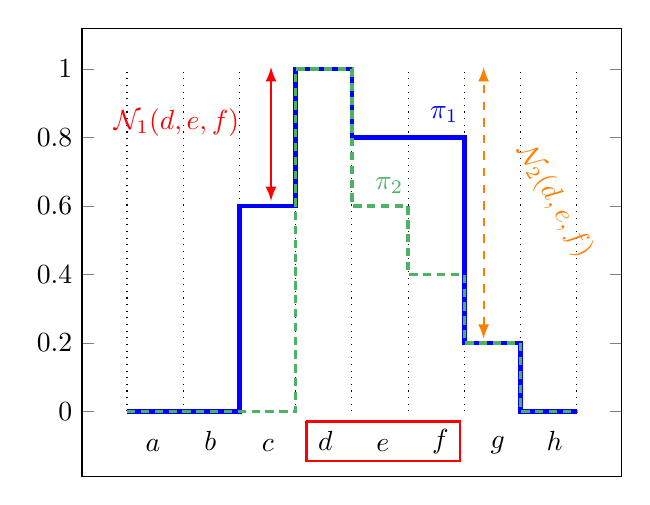
\begin{tikzpicture}
\definecolor{ggreen}{rgb}{0.3,0.7,0.4};
\begin{axis}[xtick=\empty,ymin=-0.19]
\foreach \xx in {-2,-1.5,-1,-0.5,0,0.5,1,1.5,2} {
\addplot[black,dotted] coordinates {(\xx,0) (\xx,1)};
}
\addplot[mark=none,blue, ultra thick] coordinates { (-2, 0) (-1, 0) (-1, 0.6) (-0.5, 0.6) (-0.5, 1) (0, 1) (0,0.8) (1,0.8) (1,0.2) (1.5,0.2) (1.5,0) (2,0)  };
\addplot[mark=none,ggreen, very thick, densely dashed] coordinates { (-2, 0) (-1, 0) (-1, 0 )  (-0.5, 0)   (-0.5, 1) (0, 1) (0,0.6) (0.5, 0.6) (0.5,0.4) (1,0.4) (1,0.2) (1.5,0.2) (1.5,0) (2,0)  };
\end{axis}
\node (pi1) at (4.6,4.6) { {\color{blue} $\pi_1$} };
\node (pi1) at (3.9,3.7) { {\color{ggreen} $\pi_2$} };

\node (a) at (0.9,0.4) {$a$};
\node (b) at (1.63,0.45) {$b$};
\node (c) at (2.36,0.4) {$c$};
\node (d) at (3.09,0.45) {$d$};
\node (e) at (3.82,0.4) {$e$};
\node (f) at (4.55,0.45) {$f$};
\node (g) at (5.28,0.4) {$g$};
\node (h) at (6,0.45) {$h$};

\draw[red, thick] (2.85,0.7) -- (4.8,0.7) -- (4.8,0.2) -- (2.85,0.2) -- (2.85,0.7);
\draw[<->,>=latex,red, thick] (2.4,3.5) -- (2.4,5.2);
\draw[<->,>=latex,orange, thick, dashed] (5.1,1.75) -- (5.1,5.2);

\node (nec) at (1.2,4.5) {{\color{red} $\mathcal{N}_1(\set{ d, e, f })$}};
\node (nec) at (6,3.5) [rotate=300] {{\color{orange} $\mathcal{N}_2(\set{ d, e, f })$}};

\end{tikzpicture}
\caption[Possibility distribution, Necessity measure and specificity]{Example of two possibility distributions over $\Omega=\set{a,b,c,d,e,f,g,h}$:
$\pi_1$ (solid blue line) and $\pi_2$ (dashed green one), 
with $\pi_2$ more specific than $\pi_1$.
The necessity measure $\mathcal{N}_1$ associated with $\pi_1$ 
is assessed on the event $\set{d,e,f} \subset \Omega$: 
the necessity degree is equal to $0.4 = 1-0.6$, 
as illustrated with solid red arrows.
The necessity measure is assessed on the same event: 
the necessity degree is equal to $0.8 = 1 - 0.2$, as illustrated with dashed orange arrows. }  
\label{figure_necspec}
\end{figure}

Consider now $A,B \subseteq \Omega$: whereas $\Pi \set{ A \cup B } = \max \set{ \Pi(A), \Pi(B) }$,
\[\mathcal{N}(A \cap B) = \min \set{ \mathcal{N}(A), \mathcal{N}(B) }.\] 
Indeed,
\begin{eqnarray*} 
\mathcal{N}(A \cap B) & = & 1-\Pi( \overline{A \cap B})  \\
& = & 1 - \Pi(\overline{A} \cup \overline{B})  \\
& = & 1 - \max \set{ \Pi(\overline{A}),\Pi(\overline{B}) } \\ 
& = & \min \set{1- \Pi( \overline{A}), 1-\Pi(\overline{B})  } \\
& = & \min \set{ \mathcal{N}(A),\mathcal{N}(B)}.
\end{eqnarray*}

The total ignorance is modeled by a possibility distribution $\pi$ such that $\forall \omega \in \Omega$,
$\pi(\omega)=1$ \textit{i.e.} any elementary event is possible.
As well $\forall A \subseteq \Omega$, $A \neq \Omega$, $\mathcal{N}(A)=1-\Pi(\overline{A})=1-\max_{\omega \in \overline{A}} \Pi(\omega)=0$:
apart from the universe $\Omega$,
no event is necessary. 

On the contrary, the perfect knowledge that the actual elementary event is $\omega_A \in \Omega$
is modeled by a possibility distribution $\pi$ such that $\pi(\omega_A) = 1$
and $\pi(\omega)=0$, $\forall \omega \neq \omega_A$. The necessity of the singleton $\set{\omega_A}$
is also equal to one: $\mathcal{N}(\set{\omega_A})=1-\Pi(\overline{\set{\omega_A }}) = 1$. 
The elementary event $\omega_A$ is necessary, and all the other have a null necessity degree:
if $\omega_B \neq \omega_A$, $\mathcal{N}(\set{\omega_B})=1-\Pi(\overline{\set{\omega_B }}) = 1 - \pi(\omega_A) = 0$.

These two particular cases give the intuition to formalize the knowledge, 
or the information, provided by a possibility distribution.
This idea is led by the word \textit{specificity}:
\begin{Def}[Specificity]
\label{def_specificity}
A possibility distribution $\pi_2$ is more specific (\textit{i.e.} more informative) than another possibility distribution $\pi_1$, if $\forall \omega \in \Omega$,
\[ \pi_2(\omega) \leqslant \pi_1(\omega).\]
\end{Def}
Both notions of specificity and necessity are illustrated by Figure \ref{figure_necspec}.

The main concepts of Possibility Theory have been presented.
Possibilistic planning models studied in this thesis 
are based on \textit{conditional possibility distributions}	 
and some independence assumptions, that is why
the next section focuses on these notions.

\subsection{Qualitative Conditioning and Possibilistic Independence}
\label{qualitative_indep}
In practice, two kinds of independence between variables can be distinguished. 
The first one is the \textit{decompositional independence}:
two variables $X \in \mathcal{X}$ and $Y \in \mathcal{Y}$ 
are said independent in this sense,
if the joint distribution of these two variables
can be decomposed into two marginal distributions
(one for each variable)
without losing any information
provided by the joint distribution. 
In the probabilistic framework,
variables $X$
and $Y$ are independent 
in the decompositional sense, if $\forall E \subset \mathcal{X}, F \subset \mathcal{Y}$,
\begin{equation}
\label{decompositional_indep}
\mathbb{P}(X \in E, Y \in F) = \mathbb{P}(X \in E) \cdot \mathbb{P}(Y \in F).
\end{equation}

The second kind of independence is called 
the \textit{causal independence}:
a variable $X$ is independent of a variable $Y$
in the causal sense, 
if the distribution of $X$ 
is not modified 
when something about $Y$ is learned
\textit{i.e.} there is no causality from $Y$ 
towards $X$, or yet, $Y$ does not influence $X$.
Note that this independence relation is not necessarily symetric:
``$Y$ does not influence $X$'' does not imply that 
``$X$ does not influence $Y$''.
In terms of probability measures,
the causal independence of $X$ from $Y$ can be written 
$\forall E \subset \mathcal{X}, F \subset \mathcal{Y}$,
\begin{equation}
\label{causal_indep}
\mathbb{P} \paren{ X \in E \sachant Y \in F } = \mathbb{P} ( X \in E ).
\end{equation}

In Probability Theory, both equations (\ref{decompositional_indep}) and (\ref{causal_indep})
are equivalent, if probabilities are positive, 
and then the causal independence is symetric: 
in this theory, decompositional and causal independence are equal
and called simply independence.

In Possibility Theory, Zadeh \cite{Zadeh75theconcept} introduced the \textit{non-interactivity independence},
or NI-independence, 
a decompositional independence inspired from Fuzzy Logic:
as the fuzzy generalization of the ``and'' ($\wedge$) operator is the minimum ($\min$),
if events $A$ and $B$ do not interact together,
the degree of truth of $A \cap B$ (\textit{i.e.} of the event ``A and B occur''), 
or its possibility degree,
is $\Pi(A \cap B) = \min \set{ \Pi(A), \Pi(B) }$.
The analogy is also possible with the framework of fuzzy sets,
as the fuzzy ``intersection'' ($\cap$) is represented 
by the minimum between the membership functions.
This leads to the definition of the NI-independence for variables $(X,Y) \in \mathcal{X} \times \mathcal{Y}$,
replacing the event $A$ (resp. $B$) by $\set{ X \in E } \subseteq \Omega$
with $E \subseteq \mathcal{X}$ (resp. $\set{ Y \in F } \subseteq \Omega$
with $F \subseteq \mathcal{Y}$): 
\begin{Def}[Non Interactivity Independence]
\label{def_NIindep}
Two events $A,B \subset \Omega$ are NI-independent if
\[ \Pi \paren{ A \cap B } = \min \set{ \Pi(A), \Pi(B) }. \]
Then, two variables $X \in \mathcal{X}$ and $Y \in \mathcal{Y}$ are NI-independent if  $\forall E \subset \mathcal{X}, F \subset \mathcal{Y}$,
\[  \Pi(X \in E, Y \in F ) = \min \Big\{ \Pi(X \in E), \Pi(Y \in F)  \Big\}. \] 
Finally, in terms of possibility distributions, 
it simply asserts that the joint one is equal to the minimum
between the marginal ones: $\forall x \in \mathcal{X}$, $y \in \mathcal{Y}$,
\[ \pi(x,y) = \min \set{ \pi(x), \pi(y) },  \]
where $\pi(x) = \Pi( \set{X = x} )$, $\pi(y) = \Pi( \set{Y = y} )$, and the joint possibility distribution $\pi(x,y)$ 
is $\Pi \paren{ \set{X=x} \cap \set{Y=y} }$.
\end{Def}
Note that, as $\Pi$ is a fuzzy measure, $\Pi$ is monotone, 
and then $\forall A,B \subset \Omega$,
$\Pi(A \cap B) \leqslant \Pi(A)$ and $\Pi(A \cap B) \leqslant \Pi(B)$:
thus, the inequality $\Pi(A \cap B) \leqslant \min \set{ \Pi(A), \Pi(B) }$ is always true,
with an equality when events are NI-independent.
Figure \ref{figure_noindep} illustrates a joint possibility distribution $\pi \paren{ x,y }$
over $\mathcal{X} \times \mathcal{Y}$ whose corresponding variables are not NI-independent,
whereas Figure \ref{figure_NIindep} represents a similar distribution whose variables are NI-independent.
Note that, if a joint distribution $\pi(x,y)$ is given, $\pi(x)$ can be computed from it
by marginalization using the $\max$ operator over $\mathcal{Y}$:
\begin{align*}
\pi(x)&=\Pi\Big( \set{X=x} \Big)\\ 
&=\Pi\Big( \displaystyle \cup_{y\in\mathcal{Y}} \set{ X = x } \cap \set{ Y = y } \Big) \\ 
&= \max_{y \in \mathcal{Y}} \Pi \Big( \set{ X = x } \cap \set{ Y = y } \Big) \\
&= \max_{y \in \mathcal{Y}} \pi(x,y).
\end{align*}


%%%%%%%%%%%
%%%%%%%%%%%
%%%%%%%%%%%
%%% 3D1 indep
\begin{figure}
\center
\begin{tikzpicture}

    \begin{axis}[ 
    view = {120}{70},
    xmin = 0,
    ymin = 0,
    xmax = 3,
    ymax = 3,
    zmin = 0,
    zmax = 1.1,
    unbounded coords = jump,
    colormap={pos}{color(0cm)=(white); color(6cm)=(blue)  },
ytick=\empty,
xtick=\empty,
ztick={0,0.2,0.4,0.6,0.8,1},
z post scale=2,
    ]

 \addplot3 [ultra thick]
      coordinates { (0,0,0) (0,0,0.6) (0,1,0.6) (0,1,0.4) (0,2,0.4) (0,2,1) (0,3,1) (0,3,0) };
  
 \addplot3 [ultra thick]
      coordinates { (0,0,0) (0,0,0.2) (1,0,0.2) (1,0,0.8) (2,0,0.8) (2,0,1) (3,0,1) (3,0,0) };
    
\addplot3[surf,mark=none] coordinates {

        (0,0,0.0)   (0,0,0.2)   (0,1,0.2)  (0,1,0.0)  (0,2,0.0)  (0,2,0.0)  (0,3,0.0)  (0,3,0)

        (1,0,0.0)   (1,0,0.2)   (1,1,0.2)  (1,1,0.0)  (1,2,0.0)  (1,2,0.0)  (1,3,0.0)  (1,3,0)

        (1,0,0.0)   (1,0,0.6)   (1,1,0.6)  (1,1,0.2)  (1,2,0.2)  (1,2,0.8)  (1,3,0.8)  (1,3,0)

        (2,0,0.0)   (2,0,0.6)   (2,1,0.6)  (2,1,0.2)  (2,2,0.2)  (2,2,0.8)  (2,3,0.8)  (2,3,0)

        (2,0,0.0)   (2,0,0.2)   (2,1,0.2)  (2,1,0.4)  (2,2,0.4)  (2,2,1.0)  (2,3,1.0)  (2,3,0)

        (3,0,0.0)   (3,0,0.2)   (3,1,0.2)  (3,1,0.4)  (3,2,0.4)  (3,2,1.0)  (3,3,1.0)  (3,3,0)

        (3,0,0.0)   (3,0,0.0)   (3,1,0.0)  (3,1,0.0)  (3,2,0.0)  (3,2,0.0)  (3,3,0.0)  (3,3,0)
    };
    \end{axis}

	\foreach \name/\x in {y_A/0,y_B/1,y_C/2}
	\node (xa) at (1.5*\x+0.3,-0.55*\x+0.8) {$\name$};

	\foreach \name/\x in {x_A/0,x_B/1,x_C/2}
	\node (xa) at (-0.9*\x+7,-0.9*\x+1.9) {$\name$};

	\node (pim) at (-4.5, 4.2) {$\pi \paren{ x, y } = $};

	\node (mx) at (-4.25,2) {$y_A$};
	\node (mx) at (-3.4,2) {$y_B$};
	\node (mx) at (-2.55,2) {$y_C$};

	\node (my) at (-1.7,3.5) {$x_A$};
	\node (my) at (-1.7,3) {$x_B$};
	\node (my) at (-1.7,2.5) {$x_C$};

	\node (m) at (-3.4,3) {$\begin{pmatrix}
0.2 & 0 & 0  \\
0.6 & 0.2 & 0.8 \\
0.2 & 0.4 & 1 
\end{pmatrix}$};
	\node (vx) at (6.3,6.5) {$ \pi(y) = \begin{pmatrix} 0.6 & 0.4 & 1 \end{pmatrix}$};
	\node (vy) at (-0.5,6) {$ \pi(x) = \begin{pmatrix} 0.2\\ 0.8\\ 1 \end{pmatrix}$};


\end{tikzpicture}
\caption[Joint possibility distribution without independence assumption]{Example of a joint distribution over $\mathcal{X} \times \mathcal{Y} = \set{x_A,x_B,x_C} \times  \set{y_A,y_B,y_C}$ without any independence.}  
\label{figure_noindep}
\end{figure}
%%%%%%%%%%%
%%%%%%%%%%%
%%%%%%%%%%%




%%%%%%%%%%%%%
%%%%%%%%%%%%%
%%% 3D2 indep
%%%%%%%%%%%%%
%%%%%%%%%%%%%
\begin{figure}
\center
\begin{tikzpicture}

    \begin{axis}[ 
    view = {120}{70},
    xmin = 0,
    ymin = 0,
    xmax = 3,
    ymax = 3,
    zmin = 0,
    zmax = 1.1,
    unbounded coords = jump,
    colormap={pos}{color(0cm)=(white); color(6cm)=(blue)  },
ytick=\empty,
xtick=\empty,
ztick={0,0.2,0.4,0.6,0.8,1},
z post scale=2,
    ]

 \addplot3 [ultra thick]
      coordinates { (0,0,0) (0,0,0.6) (0,1,0.6) (0,1,0.4) (0,2,0.4) (0,2,1) (0,3,1) (0,3,0) };
  
 \addplot3 [ultra thick]
      coordinates { (0,0,0) (0,0,0.2) (1,0,0.2) (1,0,0.8) (2,0,0.8) (2,0,1) (3,0,1) (3,0,0) };
    
\addplot3[surf,mark=none] coordinates {

        (0,0,0.0)   (0,0,0.2)   (0,1,0.2)  (0,1,0.2)  (0,2,0.2)  (0,2,0.2)  (0,3,0.2)  (0,3,0)

        (1,0,0.0)   (1,0,0.2)   (1,1,0.2)  (1,1,0.2)  (1,2,0.2)  (1,2,0.2)  (1,3,0.2)  (1,3,0)

        (1,0,0.0)   (1,0,0.6)   (1,1,0.6)  (1,1,0.4)  (1,2,0.4)  (1,2,0.8)  (1,3,0.8)  (1,3,0)

        (2,0,0.0)   (2,0,0.6)   (2,1,0.6)  (2,1,0.4)  (2,2,0.4)  (2,2,0.8)  (2,3,0.8)  (2,3,0)

        (2,0,0.0)   (2,0,0.6)   (2,1,0.6)  (2,1,0.4)  (2,2,0.4)  (2,2,1.0)  (2,3,1.0)  (2,3,0)

        (3,0,0.0)   (3,0,0.6)   (3,1,0.6)  (3,1,0.4)  (3,2,0.4)  (3,2,1.0)  (3,3,1.0)  (3,3,0)

        (3,0,0.0)   (3,0,0.0)   (3,1,0.0)  (3,1,0.0)  (3,2,0.0)  (3,2,0.0)  (3,3,0.0)  (3,3,0)
    };
    \end{axis}

	\foreach \name/\x in {y_A/0,y_B/1,y_C/2}
	\node (xa) at (1.5*\x+0.3,-0.55*\x+0.8) {$\name$};

	\foreach \name/\x in {x_A/0,x_B/1,x_C/2}
	\node (xa) at (-0.9*\x+7,-0.9*\x+1.9) {$\name$};

	\node (pim) at (-4.5, 4.3) {$\pi \paren{ x, y } = \min \set{ \pi(x), \pi(y) }$};
	\node (eq) at (-5.3, 3) {$=$};

	\node (mx) at (-4.25,2) {$y_A$};
	\node (mx) at (-3.4,2) {$y_B$};
	\node (mx) at (-2.55,2) {$y_C$};

	\node (my) at (-1.7,3.5) {$x_A$};
	\node (my) at (-1.7,3) {$x_B$};
	\node (my) at (-1.7,2.5) {$x_C$};

	\node (m) at (-3.4,3) {$\begin{pmatrix}
0.2 & 0.2 & 0.2  \\
0.6 & 0.4 & 0.8 \\
0.6 & 0.4 & 1 
\end{pmatrix}$};
	\node (vx) at (6.3,6.5) {$ \pi(y) = \begin{pmatrix} 0.6 & 0.4 & 1 \end{pmatrix}$};
	\node (vy) at (-0.5,6) {$ \pi(x) = \begin{pmatrix} 0.2\\ 0.8\\ 1 \end{pmatrix}$};

\end{tikzpicture}
\caption[Joint possibility distribution with NI-independence]{Example of a joint distribution over $\mathcal{X} \times \mathcal{Y} = \set{x_A,x_B,x_C} \times  \set{y_A,y_B,y_C}$ when $X$ and $Y$ are NI-independent
(no M-independence).} 
\label{figure_NIindep} 
\end{figure}
%%%%%%%%%%%
%%%%%%%%%%%
%%%%%%%%%%%



The NI-independence leads to a first qualitative possibilistic conditioning,
introduced by Hisdal \cite{Hisdal1978283}.
Indeed, the conditional possibility degree of an event $A \subset \Omega$ 
given an event $B \subset \Omega$,
namely $\Pi(A \vert B)$, can be obtained from $\Pi(B)$ and $\Pi(A \cap B)$,
as a solution of the following equation:
\begin{equation}
\label{joint_poss}
\Pi(A \cap B) = \min \Big\{ \Pi (A \vert B) , \Pi(B)  \Big\}.
\end{equation}
Intuitively, once conditioned on the event $B$,
the event $A$ (or rather ``$A \vert B$'') 
does not interact with the event $B$ anymore.
Moreover Equation \ref{joint_poss} is close to the probabilistic equation 
$\mathbb{P} \paren{ A \cap B } = \mathbb{P} (A \vert B) \cdot \mathbb{P} (B) $
which comes from the definition of the probabilistic conditioning.
Possibility Theory looks very similar to Probability Theory
observing that the addition ($+$) in Probability Theory becomes a maximum ($\max$)
in Possibility Theory, and the multiplication ($\times$)
becomes a minimum ($\min$). 
However, Quantitative Possibility Theory keeps the multiplication operator ($\times$)
for conditioning and computing joint possibility measures:
in this theory, the classical conditioning is then
equivalent to the Dempster rule of conditioning \cite{dempster1967},
an evidentialist (BFT, see Introduction) 
extension of the well-known Bayes rule.

The classical qualitative possibilistic conditioning \cite{Dubois199023},
counterpart of Bayes rule, 
is the least specific solution of Equation \ref{joint_poss}:

\vbox{
\begin{Def}[Qualitative Possibilistic Conditioning] \label{def_cond}
$\forall A,B \subset \Omega$, such that $\Pi(B)>0$, 
\begin{equation}
\label{equation_conditioning}
\Pi \paren{ A \sachant B  } = 
\left \{ 
\begin{array}{ccc}
1 & \mbox{ if } \Pi(B) = \Pi(A \cap B), \\
\Pi(A \cap B) & \mbox{otherwise}.
\end{array}
\right. 
\end{equation}
\vspace{0.5cm} \\
The conditional possibility distributions of the variable $X \in \mathcal{X}$
knowing variable $Y \in \mathcal{Y}$ is thus, $\forall x \in \mathcal{X}$, $\forall y \in \mathcal{Y}$ such that $\pi(y)>0$,

\begin{equation}
\label{equation_conddistrib}
\pi \paren{ x \sachant y } = 
\left \{ 
\begin{array}{ccc}
1 & \mbox{ if } \pi(y) = \pi(x, y), \\
\pi(x,y) & \mbox{otherwise}.
\end{array}
\right. 
\end{equation}
where $\pi \paren{ x \sachant y } = \Pi \paren{ X = x \sachant Y=y } $.
\end{Def} 
}

The meaning of the conditioning (\ref{equation_conditioning}) can be explained as follows:
when the event $A$ contains the elementary event which has the higest possibility degree in $B$,
\textit{i.e.} if $\Pi(B)=\Pi(A \cap B)$, then $\Pi \paren{ A \sachant B } = 1$.
Indeed, as conditioning on $B$ assumes that the new set of possible elementary events (universe) 
is $B$, $A$ has the maximal possibility degree among the new universe $B$:
the possibility measure conditional on $B$ is normalized,
setting to $1$ the possibility degree of most plausible events in $B$.
As qualitative possibility distributions only define a ranking between the events,
the possibility degree of events $A$ such that $\Pi(A \cap B)< \Pi(B)$ (second case of Equation \ref{equation_conditioning})
are simply set to $\Pi(A \cap B)$.
As $\min \set{ \Pi \paren{ A \sachant B }, \Pi(B) } = \Pi \paren{ A \sachant B }$,
Equation \ref{equation_conditioning} is true thanks to this choice.

Defining the qualitative possibilistic conditioning as previously (\ref{def_cond}),
the non-interactivity independence (Definition \ref{def_NIindep}) between variables $X$ and $Y$
corresponds to the fact that $\forall x,y \in \mathcal{X} \times \mathcal{Y}$ 
either the knowledge that the variable $X$ is equal to $x$ 
does not decrease the possibility degree of $Y=y$, 
or the knowledge that the variable $Y$ is equal to $y$ 
does not decrease the possibility degree of $X=x$.

\vbox{
\begin{theorem}
\label{theorem_NIequivalence}
\[ \forall (x,y) \in \mathcal{X} \times \mathcal{Y}, \ \ \ \pi \paren{ x, y } = \min \set{ \pi(x), \pi(y) } \]
\center
(non interactivity independence)\\
\vspace{0.4cm}
$\Big\Updownarrow$
\[ \forall (x,y) \in \mathcal{X} \times \mathcal{Y}, \ \ \ \pi \paren{ x } \leqslant \pi \paren{ x \sachant y } \mbox{ or } \pi \paren{ y } \leqslant \pi \paren{ y \sachant x }  \]
\begin{center}
(either the knowledge of $Y$ does not bring any knowledge about $X$, or the knowledge of $X$ doesn't bring any knowledge about $Y$.)
\end{center}
\end{theorem}
}
The proof is given in Annex \ref{theorem_NIequivalence_RETURN}.

%%%%%%%%%%%%%
%%%%%%%%%%%%%
%%% 3D3 indep
%%%%%%%%%%%%%
%%%%%%%%%%%%%
\begin{figure}
\center
\begin{tikzpicture}

    \begin{axis}[ 
    view = {120}{70},
    xmin = 0,
    ymin = 0,
    xmax = 3,
    ymax = 3,
    zmin = 0,
    zmax = 1.1,
    unbounded coords = jump,
    colormap={pos}{color(0cm)=(white); color(6cm)=(blue)  },
ytick=\empty,
xtick=\empty,
ztick={0,0.2,0.4,0.6,0.8,1},
z post scale=2,
    ]


 \addplot3 [ultra thick]
      coordinates { (0,0,0) (0,0,0.6) (0,1,0.6) (0,1,0.4) (0,2,0.4) (0,2,1) (0,3,1) (0,3,0) };
  
 \addplot3 [ultra thick]
      coordinates { (0,0,0) (0,0,0.2) (1,0,0.2) (1,0,1) (2,0,1) (2,0,1) (3,0,1) (3,0,0) };
    
\addplot3[surf,mark=none
] coordinates {

        (0,0,0.0)   (0,0,0.2)   (0,1,0.2)  (0,1,0.2)  (0,2,0.2)  (0,2,0.2)  (0,3,0.2)  (0,3,0)

        (1,0,0.0)   (1,0,0.2)   (1,1,0.2)  (1,1,0.2)  (1,2,0.2)  (1,2,0.2)  (1,3,0.2)  (1,3,0)

        (1,0,0.0)   (1,0,0.6)   (1,1,0.6)  (1,1,0.4)  (1,2,0.4)  (1,2,1.0)  (1,3,1.0)  (1,3,0)

        (2,0,0.0)   (2,0,0.6)   (2,1,0.6)  (2,1,0.4)  (2,2,0.4)  (2,2,1.0)  (2,3,1.0)  (2,3,0)

        (2,0,0.0)   (2,0,0.6)   (2,1,0.6)  (2,1,0.4)  (2,2,0.4)  (2,2,1.0)  (2,3,1.0)  (2,3,0)

        (3,0,0.0)   (3,0,0.6)   (3,1,0.6)  (3,1,0.4)  (3,2,0.4)  (3,2,1.0)  (3,3,1.0)  (3,3,0)

        (3,0,0.0)   (3,0,0.0)   (3,1,0.0)  (3,1,0.0)  (3,2,0.0)  (3,2,0.0)  (3,3,0.0)  (3,3,0)
    };


    \end{axis}

	\foreach \name/\x in {y_A/0,y_B/1,y_C/2}
	\node (xa) at (1.5*\x+0.3,-0.55*\x+0.8) {$\name$};

	\foreach \name/\x in {x_A/0,x_B/1,x_C/2}
	\node (xa) at (-0.9*\x+7,-0.9*\x+1.9) {$\name$};

	\node (pim) at (-4.5, 4.3) {$\pi \paren{ x, y } = \min \set{ \pi(x), \pi(y) }$};
	\node (eq) at (-5.3, 3) {$=$};

	\node (mx) at (-4.25,2) {$y_A$};
	\node (mx) at (-3.4,2) {$y_B$};
	\node (mx) at (-2.55,2) {$y_C$};

	\node (my) at (-1.7,3.5) {$x_A$};
	\node (my) at (-1.7,3) {$x_B$};
	\node (my) at (-1.7,2.5) {$x_C$};

	\node (m) at (-3.4,3) {$\begin{pmatrix}
0.2 & 0.2 & 0.2  \\
0.6 & 0.4 & 1 \\
0.6 & 0.4 & 1 
\end{pmatrix}$};
	\node (vx) at (6.3,6.5) {$ \pi(y) = \begin{pmatrix} 0.6 & 0.4 & 1 \end{pmatrix}$};
	\node (vy) at (-1.5,6) {$ \pi(x) = \pi \paren{x \sachant y} = \begin{pmatrix} 0.2\\ 1\\ 1 \end{pmatrix}$};

\end{tikzpicture}
\caption[Joint possibility distribution where a variable is M-independent from the other]{Example of a joint distribution over $\mathcal{X} \times \mathcal{Y} = \set{x_A,x_B,x_C} \times  \set{y_A,y_B,y_C}$ when $X$ is M-independent from $Y$.} 
\label{figure_Mindep} 
\end{figure}
%%%%%%%%%%%
%%%%%%%%%%%
%%%%%%%%%%%

Another independence called the \textit{Min-based independence},
or M-independence, comes from the conditioning (\ref{def_cond}):

\vbox{
\begin{Def}[Min-based ``Causal'' Independence]
\label{def_mcond}
The event $A \subset \Omega$ is M-independent from the event $B \subset \Omega$ if
\[ \Pi \paren{A \sachant B} = \Pi (A). \]
As well, the variable $X$ is M-independent from the variable $Y$ 
if their distributions are such that 
\[\pi \paren{ x \sachant y} = \pi \paren{x}.\]
\end{Def}
}
 
Note that, using Theorem \ref{theorem_NIequivalence},
it follows that the M-independence implies the NI-independence:
it can be also observed replacing $\Pi \paren{A \sachant B}$ by $\Pi \paren{A}$
in the equation \ref{joint_poss}, as both possibility degrees are equal. 

This independence is causal, and not symetric. Figure \ref{figure_Mindep} displays an exemple of joint distribution $\pi(x,y)$ 
such that $\pi \paren{x \sachant y} = \pi(x)$. However $\pi \paren{y \sachant x} \neq \pi(y)$:
indeed, if $X=x_A$, $Y$ is fully unknown, \textit{i.e.} $\pi \paren{ y \sachant x_A}=\begin{pmatrix} 1 & 1 & 1 \end{pmatrix}$,
if $X=x_B$, $\pi \paren{  y \sachant x_B } = \begin{pmatrix} 0.6 & 0.4 & 1 \end{pmatrix}$, and the same for $X=x_C$.
This illustrates the fact that the M-independence is not symetric.
  
The symetrized version of the M-independence is the \textit{Symetric Min-Based Independence} or MS-independence:

\vbox{
\begin{Def}[Symetric Min-Based Independence]
\label{def_mbindep}
Variables $X$ and $Y$ are said to be MS-independent if $X$ is M-independent from $Y$ and $Y$ is M-independent from $X$.
\end{Def}
}

However, this symetric independence is too restrictive: one of the variable has to be entirely unknown,
as highlighted by the following theorem.
\begin{theorem}
\label{MS2_ignor}
If $X$ and $Y$ are MS-independent, then $\forall x \in \mathcal{X}$, $\Pi \paren{ X=x } = 1$ or $\forall y \in \mathcal{Y}$, $\Pi \paren{ Y=y } = 1$.
\end{theorem}
The proof is given in Annex \ref{MS2_ignor_RETURN}.

Finally, we present a second qualitative possibilistic conditioning,
proposed in \cite{deCampos:1999:ICP:314962.314985},
based on the previous one (Definition \ref{def_cond}):
this one ensure that the posterior distribution is not less specific than the prior.
\begin{Def}[Alternative Qualitative Possibilistic Conditioning]
\label{altern_qual_cond}
This alternative conditioning is denoted by $\pi ( x \Vert y )$
and is a modified version of the classical one (Definition \ref{def_cond}): $\forall (x,y) \in \mathcal{X} \times \mathcal{Y}$,
\[ \pi ( x \Vert y ) = \left \{ \begin{array}{cc} \pi(x) & \mbox{ if } \pi \paren{ x' \sachant y } \geqslant \pi(x'), \forall x' \in \mathcal{X}, \\ \pi \paren{ x \sachant y } & \mbox{ otherwise. } \end{array} \right. \]
\end{Def}

A more general presentation of the various possibilistic conditioning and independence
and their consequences on possibilistic graphical models 
is available in the thesis of N.Ben Amor \cite{Be2002.7}.

This section just introduced that,
as the studied models will be qualitative,
the operators $\min$ and $\max$
will be present in most equations below.
Some properties about these operators,
which are used in the following sections, 
end this one.
\newpage
\begin{Property}
\label{property_minmax}
Consider the functions $f: \Omega \rightarrow \mathcal{L}$ and $\lambda \in \mathcal{L}$:
\begin{align}
\label{equationmaxmin1} \max_{\omega \in \Omega} \set{ 1 - f(\omega) } &= 1 - \min_{\omega \in \Omega} f(\omega), \\
\label{equationmaxmin2} \min_{\omega \in \Omega} \set{ 1 - f(\omega) } &= 1 - \max_{\omega \in \Omega} f(\omega), \\
\label{equationmaxmin5} \min_{\omega \in \Omega} \min \set{ f(\omega), \lambda } &= \min \set{ \min_{\omega \in \Omega} f(\omega), \lambda }, \\
\label{equationmaxmin4} \min_{\omega \in \Omega} \max \set{ f(\omega), \lambda } &= \max \set{ \min_{\omega \in \Omega} f(\omega), \lambda }, \\
\label{equationmaxmin3} \max_{\omega \in \Omega} \min \set{ f(\omega), \lambda } &= \min \set{ \max_{\omega \in \Omega} f(\omega), \lambda } \\
\label{equationargmax1} \mbox{ and } & \operatorname*{argmax}_{\omega \in \Omega} f(\omega) \subseteq \operatorname*{argmax_{\omega \in \Omega}} \min \set{ f(\omega), \lambda },\\
\label{equationmaxmin6} \max_{\omega \in \Omega} \max \set{ f(\omega), \lambda } &= \max \set{ \max_{\omega \in \Omega} f(\omega), \lambda },\\
\label{equationargmax2} \mbox{ and } & \operatorname*{argmax}_{\omega \in \Omega} f(\omega) \subseteq \operatorname*{argmax_{\omega \in \Omega}} \max \set{ f(\omega), \lambda }. 
\end{align}
\\
Let us introduce now $g:\Omega \rightarrow \mathcal{L}$ and suppose that $\exists \omega^* \in \Omega$
such that $g(\omega^*)=0$:
\begin{align}
\label{equationmaxmin7} \min_{\omega \in \Omega} \max \Big\{ \min \set{ \lambda, f(\omega) }, g(\omega) \Big\} &= \min_{\omega \in \Omega} \min \Big\{ \lambda, \max \set{ f(\omega), g(\omega)} \Big\}.
\end{align}
As well, if we introduce $h:\Omega \rightarrow \mathcal{L}$ and 
suppose that $\exists \omega^* \in \Omega$
such that $h(\omega^*)=1$,
\begin{align}
\label{equationmaxmin8} \max_{\omega \in \Omega} \min \Big\{ \max \set{ \lambda, f(\omega) }, h(\omega) \Big\} &= \max_{\omega \in \Omega} \max \Big\{ \lambda, \min \set{ f(\omega), h(\omega)} \Big\}.
\end{align}
\end{Property}
The proof is given in Annex \ref{property_minmax_RETURN}.

\subsection{Qualitative Criteria}
\label{subsection_qualcrit}

\begin{figure}[b!]
\center
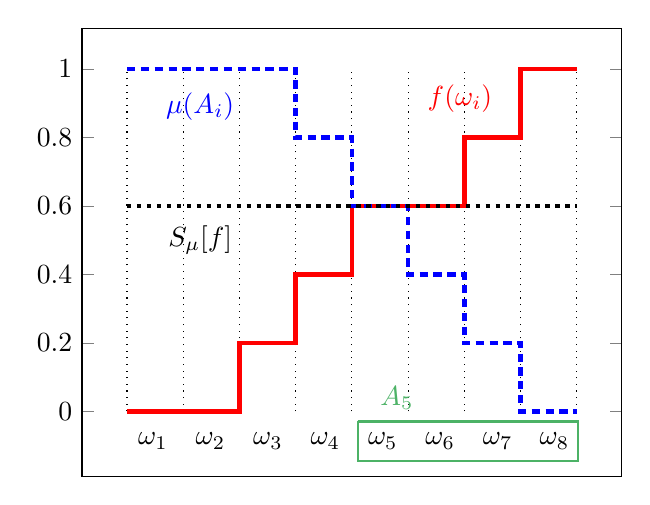
\begin{tikzpicture}
\definecolor{ggreen}{rgb}{0.3,0.7,0.4};
\begin{axis}[xtick=\empty,ymin=-0.19]
\foreach \xx in {-2,-1.5,-1,-0.5,0,0.5,1,1.5,2} {
\addplot[black,dotted] coordinates {(\xx,0) (\xx,1)};
}
\addplot[mark=none, red, ultra thick] coordinates { (-2, 0) (-1, 0) (-1, 0.2) (-0.5, 0.2) (-0.5, 0.4) (0, 0.4) (0,0.6) (1,0.6) (1,0.8) (1.5,0.8) (1.5,1) (2,1)  };
\addplot[mark=none, blue, ultra thick, densely dashed] coordinates { (-2, 1) (-1, 1) (-1, 1)  (-0.5, 1)   (-0.5, 0.8) (0, 0.8) (0,0.6) (0.5, 0.6) (0.5,0.4) (1,0.4) (1,0.2) (1.5,0.2) (1.5,0) (2,0)  };
\addplot[mark=none, black, ultra thick, dotted]%densely dashed] 
coordinates { (-2, 0.6) (2,0.6)  };
\end{axis}
\node (fff) at (4.8,4.8) { {\color{red} $f(\omega_i)$} };
\node (mumu) at (1.5,4.7) { {\color{blue} $\mu(A_i)$} };
\node (sug) at (1.5,3) {$\mathbb{S}_{\mu}[f]$};

\node (a) at (0.9,0.45) {$\omega_1$};
\node (b) at (1.63,0.45) {$\omega_2$};
\node (c) at (2.36,0.45) {$\omega_3$};
\node (d) at (3.09,0.45) {$\omega_4$};
\node (e) at (3.82,0.45) {$\omega_5$};
\node (f) at (4.55,0.45) {$\omega_6$};
\node (g) at (5.28,0.45) {$\omega_7$};
\node (h) at (6,0.45) {$\omega_8$};
\draw[ggreen, thick] (3.5,0.7) -- (6.3,0.7) -- (6.3,0.2) -- (3.5,0.2) -- (3.5,0.7);
\node (h) at (4,1) {{\color{ggreen} $A_5$}};

\end{tikzpicture}
\caption[Result of the Sugeno integral]{Illustration of the result of the Sugeno Integral: the $x$-axis represents the set $\Omega = \set{ \omega_1, \ldots, \omega_{\# \Omega} }$,
where $\forall i \in \set{1,\ldots,\# \Omega-1}$, $f(\omega_i) \leqslant f(\omega_{i+1})$.
The $y$-axis is $\mathcal{L}$. The red line represents the degrees $f(\omega_i)$, the dashed blue one represents the degrees $\mu(A_i)$ with $A_i = \set{ \omega_i, \ldots, \omega_{\# \Omega} }$,
and the black dotted one is the result of the Sugeno Integral. }  
\label{figure_sugeno}
\end{figure}

As detailed in the first section of this chapter,
the criterion used to quantify the quality of a strategy
for a given (PO)MDP
is the expectation of the reward, \textit{i.e.}
the integral of the reward function 
with respect to the probability measure.
The concept of Integral has been extended to
the framework of fuzzy measures.
When the measure is quantitative, the extension is called the \textit{Choquet Integral} \cite{Choquet1954}.
In the case of a qualitative measure, the resulting objet is the \textit{Sugeno Integral} \cite{Sugeno74}.
As the planning framework that will be studied is qualitative,
we define here the Sugeno Integral:
\begin{Def}[Sugeno Integral]
\label{sugeno_integral}
The Sugeno Integral of a function 
$f:\Omega \rightarrow \mathcal{L}$ with respect to the capacity (fuzzy measure) $\mu:2^{\Omega} \rightarrow \mathcal{L}$ is 
\begin{align} 
\label{equation_sugeno1} \mathbb{S}_{\mu} \croch{ f } &= \max_{i=1}^{\# \Omega} \min \set{ f(\omega_i), \mu(A_i) } \\
\label{equation_sugeno2} &=  \min_{i=1}^{\# \Omega} \max \set{ f(\omega_i), \mu(A_{i+1}) }
\end{align}
where $f(\omega_1) \leqslant \ldots \leqslant f(\omega_{\# \Omega})$, 
 $A_i = \set{ \omega_i, \omega_{i+1}, \ldots, \omega_{\# \Omega} }$
and $A_{\#\Omega+1} = \emptyset$.
\end{Def}
The proof of the equality is given in Annex \ref{sugeno_integral_RETURN}.

As illustrated by Figure \ref{figure_sugeno}, the Sugeno integral of $f: \Omega \rightarrow \mathcal{L}$ with respect to the fuzzy measure $\mu$
is the highest degree $\lambda \in \mathcal{L}$ 
such that the measure $\mu$ of $\set{ \omega \sachant f(\omega) \geqslant \lambda}$ 
is higher or equal to $\lambda$. As an example, the $h$-index
(or Hirsh index) is the Sugeno integral of the function $paper \mapsto \# citations$ 
with respect to the counting measure.

The Sugeno integral with respect to a possibility measure,
and the one with respect to a necessity measure,
lead to two  criteria: an optimistic and a cautious one.
The following theorem rewrites both integral in a more simple way:
\begin{theorem}[Sugeno Integrals with respect to Possibility and Necessity measures]
\label{sugenoPossNec}
\begin{align}
\label{equation_sugenoposs} \mathbb{S}_{\Pi}[f] &= \max_{i=1}^{\# \Omega} \min \set{ f(\omega_i), \pi(\omega_i) }  & \mbox{ (\textit{optimistic}), }\\
\label{equation_sugenonec} \mathbb{S}_{\mathcal{N}}[f] &= \min_{i=1}^{\# \Omega} \max \set{ f(\omega_i), 1-\pi(\omega_i) }  & \mbox{ (\textit{cautious}) }.
\end{align}
are rewritings of the Sugeno integrals with respect to 
possibility and necessity measures.
\end{theorem}
The proof is given in Annex \ref{sugenoPossNec_RETURN}.

These integrals can be seen as the possibilistic expectations of the variable $f: \Omega \rightarrow \mathcal{L}$.
Let us introduce the variable $S: \Omega \rightarrow \mathcal{S}$
whose possibility distribution is $\pi(s) = \Pi \paren{ \set{S = s} } = \Pi(\set{ \omega \in \Omega \sachant S(\omega) = s }) = \max_{\set{\omega \in \Omega \sachant S(\omega) = s} } \pi(\omega)$.
We can note for instance that the Sugeno Integral of the (classical) characteristic function of the event $\set{ S \in A}$ with $A \subseteq \mathcal{S}$,
namely $\mathds{1}_{\set{S \in A}}(\omega) =  \left \{ \begin{array}{ccc} 1 & \mbox{ if } S(\omega) \in A \\ 0 & \mbox{ otherwise } \end{array} \right.$, is equal to the possibility degree of this event:
\begin{align}
\nonumber \mathbb{S}_{\Pi} \croch{ \mathds{1}_{\set{S \in A}} } &= \max_{\omega \in \Omega} \min \set{ \mathds{1}_{ \set{S \in A}}(\omega), \pi(\omega) } \\
\nonumber&= \max_{s \in \mathcal{S}} \max_{\set{\omega \in \Omega \sachant S(\omega)=s} } \min \set{ \mathds{1}_{A}(s), \pi(\omega) } \\
\label{line3transport} &= \max_{s \in \mathcal{S}} \min \set{ \mathds{1}_{A}(s), \pi(s) } \\
\nonumber&= \max_{s \in \mathcal{S}} \left \{ \begin{array}{ccc} \pi(s) & \mbox{ if } s \in A \\ 0 & \mbox{ otherwise } \end{array} \right. \\
\label{sugenoIntCharFunc_poss} &= \max_{s \in A} \pi(s) = \Pi(S \in A).
\end{align}
where line (\ref{line3transport}) comes from equation (\ref{equationmaxmin3}) of Property (\ref{property_minmax}).
In the same way, 
\begin{align}
\nonumber \mathbb{S}_{\mathcal{N}} \croch{ \mathds{1}_{\set{S \in A}} } &= \min_{s \in \mathcal{S}} \max \set{ \mathds{1}_{A}(s), 1 - \pi(s) } \\
\label{line3nec} &= \min_{s \in \mathcal{S}} \set{ 1 - \min \set{ 1 - \mathds{1}_{A}(s), \pi(s) } } \\
\label{line4nec} &= 1 -\max_{s \in \mathcal{S}} \min \set{ \mathds{1}_{\overline{A}}(s), \pi(s) } \\
\nonumber &= 1 - \max_{s \in \overline{A}} \pi(s) = 1 - \Pi \paren{ \set{S \in \overline{A}} } = \mathcal{N} \paren{ \set{S \in A}}.
\end{align}
where lines (\ref{line3nec}) and (\ref{line4nec}) come from equation 
(\ref{equationmaxmin1}) and (\ref{equationmaxmin2}) 
of Property (\ref{property_minmax}).
These remarks are the counterparts of the probabilistic equality $\mathbb{E} \croch{ \mathds{1}_{\set{S \in A}} } = \mathbb{P}( \set{S\in A})$.

Qualitative Possibilistic Decision Criteria,
\textit{i.e.} functions $\mathcal{A} \rightarrow \mathcal{L}$ 
measuring the accuracy of actions given a possibilistic and a preference model,
have been proposed in \cite{DBLP:journals/ijar/SabbadinFL98,DBLP:journals/eor/DuboisPS01,Dubois95possibilitytheory},
based on Sugeno integrals (\ref{equation_sugenoposs}) and (\ref{equation_sugenonec}).
Let us recall that the set $\mathcal{S}$ (resp. $\mathcal{A}$) 
is as previously the finite set of system states $s$ (resp. of actions $a$).
The variable representing the system state is $S \in \mathcal{S}$.
Let $\big(\pi_a\big)_{a \in \mathcal{A}}$ be a family of 
possibility distributions over $\mathcal{S}$,
\textit{i.e.} $\forall a \in \mathcal{A}$, $\pi_a(s) = \Pi_a( \set{S = s} )$
is the possibility degree of the situation $\set{S=s} \subset \Omega$ after selecting action $a \in \mathcal{A}$. 
Let function $\rho: \mathcal{S} \rightarrow \mathcal{L}$ be the preference function, 
defining the preference degree of each system state $s \in \mathcal{S}$.

\begin{Def}[Qualitative Decision Criteria]
Let $\pi_a$ be the possibility distribution 
describing the uncertainty about the system state
given that action $a \in \mathcal{A}$ has been selected, 
and $\rho(s)$ the preference of the system state $s \in \mathcal{S}$.
Using the formula (\ref{equation_sugenoposs}) with $f=\rho(S)$, 
the Sugeno integral of the preference with respect to the possibility measure $\Pi_a$ 
leads to an optimistic criteria for $a \in \mathcal{A}$:
\label{def_qualcrit}
\begin{align}
\label{equation_critopt} \mathbb{S}_{\Pi_a}[\rho(S)] &= \max_{s \in \mathcal{S}} \min \set{ \rho(s), \pi_a(s) }.
\end{align}
As well, using the formula (\ref{equation_sugenonec}) with $f=\rho(S)$, 
the Sugeno integral of the preference with respect to the necessity measure associated to $\Pi_a$, $\mathcal{N}_a$, 
leads to a cautious criteria for $a \in \mathcal{A}$:
\begin{align}
\label{equation_critpess} \mathbb{S}_{\mathcal{N}_a}[\rho(S)] &= \min_{s \in \mathcal{S}} \max \set{ \rho(s), 1-\pi_a(s) }.
\end{align}
\end{Def}

These criteria can be understood best with the fuzzy sets vision:
a possibility distribution $\pi_a: \mathcal{S} \rightarrow \mathcal{L}$ 
is the characteristic (or membership) function of the fuzzy set of the possible system states 
after selecting $a \in \mathcal{A}$,
denoted by $\textgoth{T}^{a}$ \textit{i.e.} $\pi(s) = \mathds{1}_{\textgoth{T}^a}$(s).
The preference function $\rho: \mathcal{S} \rightarrow \mathcal{L}$ 
can also be viewed as the characteristic function 
of the fuzzy set denoted by $\textgoth{R}$ representing the preferred system states:
$\rho(s) = \mathds{1}_{\textgoth{R}}(s)$.
Finally, the characteristic function of the fuzzy set 
of plausible and preferred states after selecting action $a \in \mathcal{A}$, \textit{i.e.} $\textgoth{T}^a \cap \textgoth{R}$,
is $\mathds{1}_{\textgoth{T}^a \cap \textgoth{R}} = \min \set{ \mathds{1}_{\textgoth{T}^a}, \mathds{1}_{\textgoth{R}} }
= \min \set{ \pi_a, \rho }$.

An action $a \in \mathcal{A}$ maximizing the optimistic criterion (\ref{equation_critopt}),
is thus an action that maximizes the highest membership degree of $\textgoth{T}^a \cap \textgoth{R}$,
\textit{i.e.} of the fuzzy set of possible and preferred states.
This criterion is optimistic because it maximizes
the degree of the best situation, but does not ensure that 
unwanted states are avoided by the system.
 
The characteristic function of the complementary set of $\textgoth{T}^a$, denoted by $\overline{\textgoth{T}^a}$ 
is $\mathds{1}_{\overline{\textgoth{T}^a}} = 1 - \mathds{1}_{\textgoth{T}^a} = 1- \pi_a$:
the fuzzy set of implausible system state.
An action $a \in \mathcal{A}$ maximizing the pessimistic criterion (\ref{equation_critpess}),
is thus an action that maximizes the lowest membership degree of $\overline{\textgoth{T}^a} \cup \textgoth{R}$,
\textit{i.e.} of the fuzzy set of the system states which are implausible or preferred.
An action that maximizes the lowest degree of this fuzzy set,
tries to make all the system states either implausible or preferred,
\textit{i.e.} to ensure that if any system state is plausible it is preferred:
it maximizes the ``degree'' of the inclusion $\textgoth{T} \subseteq \textgoth{R}$.

\begin{figure} 
\center
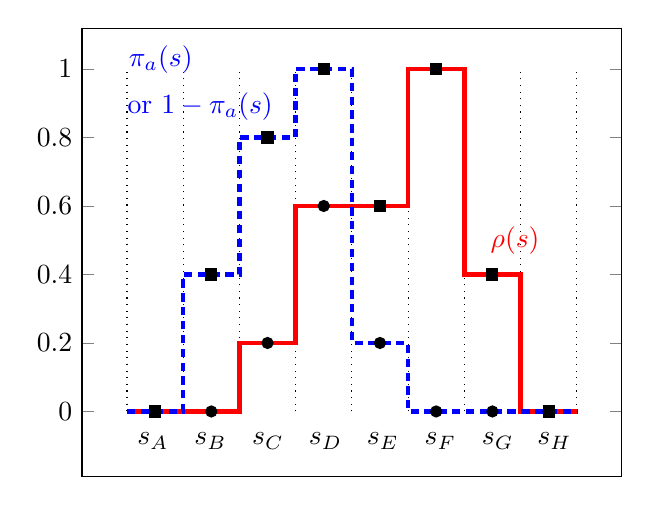
\begin{tikzpicture}
\definecolor{ggreen}{rgb}{0.3,0.7,0.4};
\begin{axis}[xtick=\empty,ymin=-0.19]
\foreach \xx in {-2,-1.5,-1,-0.5,0,0.5,1,1.5,2} {
\addplot[black,dotted] coordinates {(\xx,0) (\xx,1)};
}
\addplot[mark=none, red, ultra thick] coordinates { (-2, 0) (-1, 0) (-1, 0.2) (-0.5, 0.2) (-0.5, 0.6) (0.5,0.6) (0.5,1) (1,1) (1,0.4) (1.5,0.4) (1.5,0) (2,0)  };
\addplot[mark=none, blue, ultra thick, densely dashed] coordinates { (-2, 0.0) (-1.5, 0.0) (-1.5, 0.4)  (-1, 0.4) (-1, 0.8) (-0.5,0.8) (-0.5, 1) (0, 1) (0,0.2) (0.5, 0.2) (0.5,0.0) (1,0.0) (1,0.0) (1.5,0.0) (1.5,0) (2,0)  };

\addplot[mark =*, only marks] coordinates { (-1.75, 0.0) (-1.25, 0.0) (-0.75, 0.2)  (-0.25, 0.6) (0.25, 0.2) (0.75,0) (1.25, 0) (1.75, 0)};
\addplot[mark=square*, only marks] coordinates { (-1.75, 0.0) (-1.25, 0.4) (-0.75,0.8) (-0.25,1) (0.25,0.6) (0.75,1) (1.25,0.4) (1.75,0)  };
\end{axis}
\node (fff) at (1,5.3) { {\color{blue} $\pi_a(s)$} };
\node (fff) at (1.5,4.7) { {\color{blue} or $1- \pi_a(s)$} };
\node (mumu) at (5.5,3) {  {\color{red} $ \rho(s)$} };

\node (a) at (0.9,0.45) {$s_A$};
\node (b) at (1.63,0.45) {$s_B$};
\node (c) at (2.36,0.45) {$s_C$};
\node (d) at (3.09,0.45) {$s_D$};
\node (e) at (3.82,0.45) {$s_E$};
\node (f) at (4.55,0.45) {$s_F$};
\node (g) at (5.28,0.45) {$s_G$};
\node (h) at (6,0.45) {$s_H$};

\end{tikzpicture}
\caption[Qualitative criteria]{Illustration of the qualitative criteria. The solid red line is $\rho(s) = \mathds{1}_{\textgoth{R}}(s)$. 
The dashed blue line may represent $\pi_a(s) = \mathds{1}_{\textgoth{T}^a}(s)$,
and the black circles represent the characteristic function of the intersection $\mathds{1}_{\textgoth{T}^a \cap \textgoth{R}}(s) = \min \set{ \rho(s),\pi_a(s) }$.
Actions maximizing the optimistic criterion (\ref{equation_critopt}),
maximizes the highest membership degree $\max_{s \in \mathcal{S}} \mathds{1}_{\textgoth{T}^a \cap \textgoth{R}}(s)$,
which is here equal to $0.6$, the degree of $s_D$. 
The dashed blue line may also represend $1 - \pi_a(s) = \mathds{1}_{\overline{\textgoth{T}^a}}(s)$,
and the black squares represent the characteristic function of the union 
 $\mathds{1}_{\overline{\textgoth{T}^a} \cup \textgoth{R}}(s) = \max \set{\rho(s), 1-\pi_a(s) }$.
Actions maximizing the pessimistic criterion (\ref{equation_critpess}),
maximizes the lowest membership degree $\min_{s \in \mathcal{S}} \mathds{1}_{\overline{\textgoth{T}^a} \cup \textgoth{R}}(s)$,
which is here equal to $0$, as $s_A$ and $s_H$ are totally possible and unpleasant.}  
\label{figure_criteria} 
\end{figure}

Note that, for a function $f: \mathcal{A} \rightarrow \mathcal{L}$,
$\operatorname*{argmax}_{a \in A} f(a) = 1 - \operatorname*{argmin}_{a \in A} f(a)$,
which can be shown as equation (\ref{equationmaxmin2}) of Property \ref{property_minmax}.
Thus, 
\[\operatorname*{argmax}_{a \in A} \set{ \displaystyle \min_{s \in  \mathcal{S}} \max\set{ \rho(s),  1- \pi_a(s) } } = \operatorname*{argmin}_{a \in A} \set{ \displaystyle 1 - \min_{s \in \mathcal{S}} \max\set{ \rho(s), 1 - \pi_a(s) } }.\]
As  $1 - \displaystyle \min_{s \in \mathcal{S}} \max\set{ \rho(s), 1 - \pi_a(s) } = \displaystyle \max_{s \in \mathcal{S}} \Big\{ 1 - \max\set{ \rho(s), 1 - \pi_a(s)} \Big\} =  \displaystyle \max_{s \in \mathcal{S}} \min\{ 1-\rho(s), \pi_a(s)  \}$ 
(see equations (\ref{equationmaxmin1}) and (\ref{equationmaxmin2}) of Property \ref{property_minmax}),
the action $a \in \mathcal{A}$ minimizes the highest membership degree 
of the fuzzy set $\textgoth{T}^a \cap \overline{\textgoth{R}}$,
\textit{i.e.} the fuzzy set of plausible and unwanted system states:
the pessimistic criterion tries to keep down all membership degrees of this set. 

The pessimistic criterion (\ref{equation_critpess}) tends to avoid unwanted system states,
whereas the optimistic criterion (\ref{equation_critopt}) wants to make possible 
that the system reaches preferred ones.
Figure (\ref{figure_criteria}) illustrates the result of the criteria for a given action $a\in\mathcal{A}$.

The following toy example, illustrated in Figure \ref{figure_example} 
is meant to present the two criteria in practice:
let the set of system states $\mathcal{S}$ be $\set{ s_A , s_B , s_C }$
and the set of actions $\mathcal{A} = \set{ a_1 , a_2 }$. 
The preference model and the uncertainty model are described respectively by $\rho$ and $\paren{\pi_a}_{a \in \mathcal{A}}$:
\begin{itemize}
\item[$\bullet$] $1 = \rho(s_A) > \rho(s_B) > \rho(s_C) = 0$;
\item[$\bullet$] selecting action $a_1$, $\pi_{a_1}(s_A) = \pi_{a_1}(s_C) = 1$, and $\pi(s_B) = 0$;
\item[$\bullet$] selecting action $a_2$, $\pi_{a_2}(s_A) = \pi(s_C) = 0$, and $\pi(s_B) = 1$, \textit{i.e.}
the system is in state $s_B$ deterministically.
\end{itemize}
As $\min \set{ \rho(s), \pi_{a_1}(s) } = \left \{  \begin{array}{ll}
1 & \mbox{ if } s=s_A, \\
0 & \mbox{ otherwise. }
\end{array} \right.  $,
the optimistic criterion is equal to $S_{\Pi_{a_1}} \croch{ r(S) } = 1$
for $a_1$.
Now, as $\min \set{ \rho(s), \pi_{a_2}(s) } = \left \{  \begin{array}{ll}
\rho(s_B) & \mbox{ if } s=s_B, \\
0 & \mbox{ otherwise. }
\end{array} \right.  $,
the optimistic criterion is equal to $S_{\Pi_{a_2}} \croch{ r(S) } = \rho(s_B)$
for $a_2$. Thus, as $\rho(s_B)<1$, $a_1$ maximizes the optimistic criterion (\ref{equation_critopt}).

\begin{figure}
\center
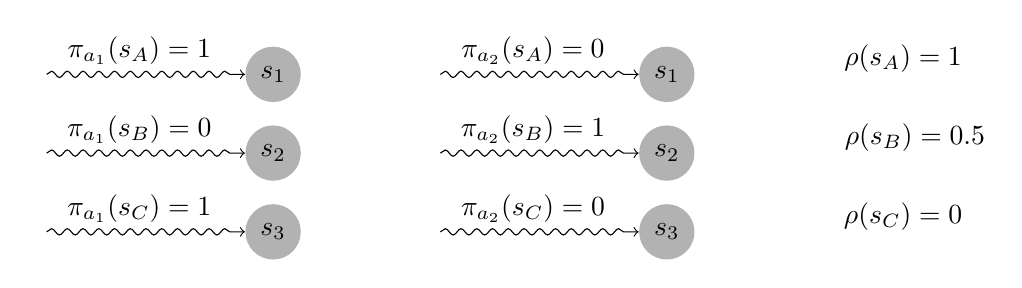
\begin{tikzpicture} 
\tikzstyle{vertex}=[circle,fill=black!30,minimum size=20pt,inner sep=0pt]
\node[vertex] (G1) at (0,1) {$s_1$};
\node[vertex] (G2) at (0,0) {$s_2$};
\node[vertex] (G3) at (0,-1) {$s_3$};
\node (G1b) at (-3,1) {};
\node (G2b) at (-3,0) {};
\node (G3b) at (-3,-1) {};

\node (poss1) at (-1.7,1.3) {$\pi_{a_1}(s_A)=1$};
\node (poss2) at (-1.7,0.3) {$\pi_{a_1}(s_B)=0$};
\node (poss3) at (-1.7,-0.7) {$\pi_{a_1}(s_C)=1$};
\draw[->,decorate,decoration={snake,amplitude=.4mm,segment length=2mm,post length=1mm}] (G1b) to (G1);
\draw[->,decorate,decoration={snake,amplitude=.4mm,segment length=2mm,post length=1mm}] (G2b) to (G2);
\draw[->,decorate,decoration={snake,amplitude=.4mm,segment length=2mm,post length=1mm}] (G3b) to (G3);

\node[vertex] (GG1) at (5,1) {$s_1$};
\node[vertex] (GG2) at (5,0) {$s_2$};
\node[vertex] (GG3) at (5,-1) {$s_3$};
\node (GG1b) at (2,1) {};
\node (GG2b) at (2,0) {};
\node (GG3b) at (2,-1) {};

\node (poss1) at (3.3,1.3) {$\pi_{a_2}(s_A)=0$};
\node (poss2) at (3.3,0.3) {$\pi_{a_2}(s_B)=1$};
\node (poss3) at (3.3,-0.7) {$\pi_{a_2}(s_C)=0$};
\draw[->,decorate,decoration={snake,amplitude=.4mm,segment length=2mm,post length=1mm}] (GG1b) to (GG1);
\draw[->,decorate,decoration={snake,amplitude=.4mm,segment length=2mm,post length=1mm}] (GG2b) to (GG2);
\draw[->,decorate,decoration={snake,amplitude=.4mm,segment length=2mm,post length=1mm}] (GG3b) to (GG3);

\node (mu1) at (8,1.2) {$\rho(s_A)=1$};
\node (mu2) at (8.15,0.2) {$\rho(s_B)=0.5$};
\node (mu3) at (8,-0.8) {$\rho(s_C)=0$};
\end{tikzpicture}
\caption[Example of a situation to illustrate qualitative criteria]{Illustration of the situation in the example of Section \ref{subsection_qualcrit}
about qualitative criteria. Action $a_1$ maximizes the optimistic criterion (\ref{equation_critopt}),
which can lead to the best state ($s_A$), but also the worst ($s_C$).
On the contrary, action $a_2$ maximizes the pessimistic criterion (\ref{equation_critpess})
since the worst state is not reachable with this action.}  \label{figure_example}
\end{figure}

The optimistic criterion is maximized by the action $a_1$, 
because with this action, the best system state, $s_A$, is entirely possible.
However, this action makes also the worst system state, $s_C$ entirely possible:
state $s_A$ is not necessary at all: 
$\mathcal{N}(\set{ s_A }) = 1-\pi \paren{\set{ s_B , s_C }} = 1 - \max \paren{ \pi(s_B), \pi(s_C)} = 0$. 
A more cautious action is $a_2$, whose the preference of the reached state ($s_B$)
is lower than $1$, but certain.

As expected, the action $a_2$ maximizes the cautious criterion (\ref{equation_critpess}):
$\max \set{ \rho(s), 1-\pi_{a_1}(s) } = \left \{ \begin{array}{ll}
1 & \mbox{ if } s=s_A \mbox{ or } s_B, \\
0 & \mbox{ otherwise. }
\end{array}  \right.$ and then the cautious criterion 
is equal to $0$ for $a_1$.
It is greater with $a_2$: 
$\max \set{ \rho(s), \pi_{a_2}(s) } = \left \{ \begin{array}{ll}
1 &  \mbox{ if } s=s_A \mbox{ or } s_C, \\
\rho(s_B) & \mbox{ otherwise. }
\end{array}  \right.$ and thus the criterion is equal to $\rho(s_B)>0$ for $a_2$.
This choice is more cautious since $\mathcal{N}_{a_2}(\set{ s_B} ) = 1-\Pi \paren{ \set{ s_A , s_C } } = 1$, 
\textit{i.e.} the preference of the state will be $\rho(s_B)$ with certainty.

This section ends with a remark about this qualitative framework:
possibility degrees are compared to preference degrees in the presented criteria.
This requests a \textit{commensurability} assumption,
\textit{i.e.} these comparisons must mean something. 
When values of $\rho$ are in $\set{ 0 , 1 }$, 
this assumption is not necessary as system states with a preference of $1$
are the goals, and other states are not.
How to model problems in practice 
with these settings will be detailed in experimental parts.
%%%%%%%%%%%%%%%%%%%%%%%%%%%%%%%%%%%%%%%%%%%%%%%%%%%%%%
\subsection{$\pi$-MDPs}
\label{subsection_piMDPs}
This model, presented in \cite{Sabbadin2001287,conf/ecai/Sabbadi00,Sabbadin:1999:pipomdp}, 
is a qualitative possibilistic version of the probabilistic MDPs detailed in Section \ref{subsection_MDP},
based on the criteria (optimistic and pessimistic) presented in Section \ref{subsection_qualcrit}:
this version is called \textit{Qualitative Possibilistic Markov Decision Process}, or $\pi$-MDP.

The finite set of system states, describing the agent and its environment, 
remains denoted by $\mathcal{S}$, as seen in Section \ref{subsection_MDP} 
where probabilistic MDPs are presented.
The finite set of action is always $\mathcal{A}$ 
and $\mathcal{L}$ is the possibility scale $\set{ 0, \frac{1}{k}, \ldots, 1 }$,
with $k\geqslant2$.

As in the probabilistic case, this model considers that
successive system states, 
represented by the sequence of variables $(S_t)_{t \in \mathbb{N}}$
with $S_t \in \mathcal{S}$ $\forall t \geqslant 0$, is Markovian. 
In this qualitative possibilistic framework, 
it means that the sequence $(S_t)_{t \in \mathbb{N}}$ is such that
$\forall t \geqslant 0,  \forall (s_0,s_1,\ldots,s_{t+1}) \in \mathcal{S}^{t+2}$
and for each action sequence of action $(a_t)_{t\geqslant 0} \in \mathcal{A}^{\mathbb{N}}$, 
$S_{t+1}$ is $M$-independent (see Definition \ref{def_mcond}) from variables $\set{ S_0, \ldots, S_{t-1} }$,
conditioned on $\set{S_t = s}$ and $a_t$: 
\begin{equation}
\label{equation_possmarkov}
  \Pi \Big( \ S_{t+1}=s_{t+1} \ \Big\vert \ S_t=s_t, a_t \ \Big) = \Pi \Big( \ S_{t+1}=s_{t+1} \ \Big\vert \ S_t=s_t, S_{t-1}=s_{t-1}, \ldots, S_0=s_0, (a_t)_{t \geqslant 0} \ \Big).
\end{equation}
Using this property, dynamics of the system are fully described 
with possibilistic transitions $\pi_t \paren{ s' \sachant s, a } = \Pi \Big( \ S_{t+1}=s' \ \Big\vert \ S_t=s, a \ \Big)  \in \mathcal{L}$:
$\forall t \geqslant 0$, $(s,s') \in \mathcal{S}^2$ and $a \in \mathcal{A}$,
$\pi_t \paren{ s' \sachant s, a }$ is the possibility degree, that at time step $t$, 
the system reaches the state $s'$ when the agent selects action $a$, 
conditioned to the fact that the current state is $s$.
Finally a $\pi$-MDP is entirely defined with the sequence of preference functions $(\rho_t)_{t=0}^{H-1}$,
where $\forall s \in \mathcal{S}$, $\forall a\in \mathcal{A}$, 
$\rho_t(s,a)$ is the preference degree when the system state is $s$ and the agent selects action $a$ at time step $t$.
The final preference function, $\Psi$, gives for each system state $s \in \mathcal{S}$, the preference degree
if $S_H = s$: $\Psi(s)$. With the previous notations for the preference functions,
$\Psi(s)=\rho_{H}(s,a)$, $\forall s \in \mathcal{S}$, $a \in \mathcal{A}$.
Figure \ref{fig_mdp} in the MDP section (Section \ref{subsection_MDP})
is a good representation of a $\pi$-MDP, replacing rewards by preferences,
and probability distributions by possibility distributions.

In order to easily derive the MDP criteria 
from the qualitative possibilistic criteria (\ref{equation_critopt}) and (\ref{equation_critpess}), 
let us introduce, for an horizon $H\geqslant0$, 
a \textit{$H$-length trajectory} $\mathcal{T} = (s_1,\ldots,s_{H})$,
and $\mathcal{T}_H = \mathcal{S}^{H}$ the set of such trajectories.
A decision rule is denoted by $\delta: \mathcal{S} \rightarrow \mathcal{L}$, 
and a $H$-length strategy is a sequence of decision rules $\delta_t$: $(\delta_t)_{t=0}^{H-1}$.
The set of all the $H$-length strategies is denoted by $\Delta_H$.
In \cite{Sa1998.16}, for a given $H$-length strategy $(\delta) \in \Delta_H$,
a given sequence of system states $\mathcal{T} = (s_1,\ldots,s_H) \in \mathcal{T}_H$, 
and a given initial state $s_0 \in \mathcal{S}$,
the \textit{preference of an $H$-length trajectory from $s_0$} 
is defined as the lowest preference degree along $s_0$ and the trajectory:
\[ \rho \Big( \mathcal{T}, (\delta) \Big) = \min \set{ \min_{t=0}^{H-1} \rho\Big(s_t,\delta_t(s_t)\Big), \Psi(s_H)}.\]
This is the possibilistic counterpart of the sum $\sum_{t=0}^{H-1} r_t \Big( S_t,d_t(S_t) \Big) + R(S_H)$,
reward aggregation of the probabilistic framework. Note that any preference aggregation of the qualitative possibilistic framework
has to result in a degree $\lambda \in \mathcal{L}$.

Using the Markov property of this system state process,
for a given initial system state $s_0 \in \mathcal{S}$, 
a horizon $H \in \mathbb{N}$,
and a strategy $(\delta_t)_{t=0}^{H-1}$, 
the possibility degree of the trajectory $\mathcal{T} = (s_1, \ldots, s_H)$ is
\begin{equation}
\label{equation_possdistribtraj}
\Pi \paren{ S_H=s_h, S_{H-1}=s_{h-1}, \ldots, S_1 = s_1 \Big\vert S_0 = s_0, \big(\delta_t\big)_{t=0}^{H-1} } = \min_{t=0}^{H-1} \pi_{t+1} \Big( s_{t+1} \Big\vert s_{t}, \delta_{t}(s_{t}) \Big)
\end{equation}
denoted by $\pi \Big( \mathcal{T} \Big\vert s_0, (\delta) \Big)$.

The Sugeno integral of the preference of the trajectory
with respect to this distribution
is denoted by 
\[\mathbb{S}_{\Pi} \croch{ \rho \Big( \mathcal{T}, (\delta) \Big) \sachant S_0 = s_0, (\delta) } = \mathbb{S}_{\Pi} \croch{ \displaystyle \min \set{ \min_{t=0}^{H-1} \rho \Big(S_t,\delta_t(S_t) \Big), \Psi(S_H) } \sachant S_0 = s_0, (\delta) }\]
and defines the optimistic criterion defining optimal strategies,
\textit{i.e.} an optimistic value function:
\begin{align} 
\overline{U_H} \Big( s_0,(\delta_t)_{t=0}^{H-1} \Big) &= \max_{\mathcal{T} \in \mathcal{T}_H} \min \set{ \rho \Big( \mathcal{T}, (\delta) \Big), \pi \Big( \mathcal{T} \Big\vert s_0, (\delta) \Big) }. \label{equation_optqualvalue} 
\end{align}
It is equivalent to the optimistic qualitative possibilistic criterion (\ref{equation_critopt}),
however, the expectation is over trajectories $\mathcal{T}_H$, and the preference depends on the strategy.
%$= \mathbb{S}_{\Pi} \croch{ \displaystyle \min \set{ \min_{t=0}^{H-1} \rho \Big(S_t,\delta_t(S_t) \Big), \Psi(S_H) } \sachant S_0 = s_0 }$
%Formally, the optimistic value function is the Sugeno integral
%of the trajectory preference with respect to 
%the possibility measure over trajectories .
The \textit{optimal optimistic strategy} $\overline{\delta^*}$ is the strategy
maximizing the optimistic value function (\ref{equation_optqualvalue}),
and the \textit{optimal optimistic value function}
is the maximal optimistic value function among strategies $(\delta) \in \Delta_H$:
\begin{Def}[Optimal Optimistic Value Function and Strategy]
$\forall s \in \mathcal{S}$,
\begin{align} 
\label{equation_optqualvaluestar} \overline{U_H^*}(s) &= \max_{(\delta) \in \Delta_H} \set{ \overline{U_H} \Big(s,(\delta)\Big) } & \mbox{ (optimal optimistic value function), } \\
\label{equation_optqualstratstar} \overline{\delta^*}(s) &\in \operatorname*{argmax}_{(\delta) \in \Delta_H} \set{ \overline{U_H} \Big(s,(\delta)\Big) } & \mbox{ (optimal optimistic strategy). } 
\end{align}
\end{Def}

As well, the pessimistic qualitative possibilistic criterion (\ref{equation_critpess})
leads to a cautious criterion for strategies: 
the pessimistic value function is
the Sugeno integral of the preference trajectory 
with respect to the necessity measure
which comes from the possibility distribution over trajectories $\mathcal{T}_H$ (\ref{equation_possdistribtraj}) 
with the strategy $(\delta) \in \Delta_H$:
\begin{align} 
 \underline{U_H} \Big( s_0,(\delta_t)_{t=0}^{H-1} \Big) &= \min_{\mathcal{T} \in \mathcal{T}_H} \max \set{ \rho \Big( \mathcal{T},  (\delta) \Big), 1 - \pi \Big( \mathcal{T} \Big\vert s_0, (\delta) \Big) }. \label{equation_pessqualvalue}
\end{align}
denoted by $\mathbb{S}_{\mathcal{N}} \croch{ \rho \Big( \mathcal{T},  (\delta) \Big) \sachant S_0 = s, (\delta) }$.
As previously for the optimistic case,
the \textit{optimal cautious strategy} $\underline{\delta^*}$ is the strategy
maximizing the pessimistic value function (\ref{equation_pessqualvalue}),
and the \textit{optimal pessimistic value function}
 is the maximal pessimistic value function among strategies $(\delta) \in \Delta_H$:
\\
\\

\begin{Def}[Optimal Pessimistic Value Function and Strategy]
$\forall s \in \mathcal{S}$,
\begin{align} 
\label{equation_pessqualvaluestar} \underline{U_H^*}(s) &= \max_{(\delta) \in \Delta_H} \set{ \underline{U_H} \Big(s,(\delta)\Big) } & \mbox{ (optimal pessimistic value function), } \\
\label{equation_pessqualstratstar} \underline{\delta^*}(s) &\in \operatorname*{argmax}_{(\delta) \in \Delta_H} \set{ \underline{U_H} \Big(s,(\delta)\Big) } & \mbox{ (optimal pessimistic strategy). } 
\end{align}
\end{Def}




As for the probabilistic MDPs (see Section \ref{subsectionDP} Theorem \ref{thm_mdp_finiteH}),
optimal value functions and strategies can be computed with Dynamic Programming:
\begin{theorem}[Dynamic Programming for $\pi$-MDPs]
\label{DPpiMDP}
The optimal optimistic criterion and an associated optimal strategy 
can be computed as follows: $\forall s \in \mathcal{S}$,
\begin{align}
\nonumber 
\overline{U_0^*}(s) & = \Psi(s), \mbox{\hspace{1cm} and, $\forall 1 \leqslant i \leqslant H$,} \\
\label{equation_recursiveopt} 
\overline{U_{i}^*}(s)& = \max_{a \in \mathcal{A}} \min \set{ \rho_{H-i}(s,a), \max_{s' \in \mathcal{S}} \min \set{ \pi_{H-i} \paren{ s' \sachant s, a  } , \overline{U^*_{i-1}}(s') }  }.
\end{align}
\begin{eqnarray}
\label{equation_recursiveoptstrat} 
\overline{\delta^*_{H-i}}(s) \in \operatorname*{argmax}_{a \in \mathcal{A}} \min \set{ \rho_{H-i}(s,a), \max_{s' \in \mathcal{S}} \min \set{ \pi_{H-i} \paren{ s' \sachant s, a  } , \overline{U^*_{i-1}}(s') }  }.
\end{eqnarray}
As well, the optimal pessimistic criterion and an associated optimal strategy 
can be computed as follows: $\forall s \in \mathcal{S}$,
\begin{align}
\nonumber 
\underline{U_0^*}(s) & = \Psi(s), \mbox{\hspace{1cm} and, $\forall 1 \leqslant i \leqslant H$,} \\
\label{equation_recursivepess} 
\underline{U_{i}^*}(s)& = \max_{a \in \mathcal{A}} \min \set{ \rho_{H-i}(s,a), \min_{s' \in \mathcal{S}} \max \set{ 1 - \pi_{H-i} \paren{ s' \sachant s, a  } , \underline{U^*_{i-1}}(s') }  }.
\end{align}
\begin{eqnarray}
\label{equation_recursivepessstrat} 
\underline{\delta^*_{H-i}}(s) \in \operatorname*{argmax}_{a \in \mathcal{A}} \min \set{ \rho_{H-i}(s,a), \min_{s' \in \mathcal{S}} \max \set{ 1 - \pi_{H-i} \paren{ s' \sachant s, a  } , \underline{U^*_{i-1}}(s') }  }.
\end{eqnarray}
\end{theorem}
The proof is given in Annex \ref{DPpiMDP_RETURN}.

In this theorem, the horizon $i$ is the opposite modulo $H$ 
of the stage of the process $t$: during execution,
$\delta_{t} = \delta_{H-i}$ is used at time step $t$,
\textit{i.e.} when it remains $i$ steps. 
These Dynamic Programming formulae 
lead to the optimistic algorithm, Algorithm \ref{dynamic_programming_pimdp} and 
the pessimistic one Algorithm \ref{dynamic_programming_pimdppess},
qualitatif possibilistic counterpart of Algorithm \ref{dynamic_programming_mdp}
for finite horizon probabilistic MDPs.
\begin{algorithm}
 \caption{Dynamic Programming Algorithm for Optimistic $\pi$-MDP} \label{dynamic_programming_pimdp}
$\overline{U^*_0} \gets \Psi$;\\
\For{$i \in \set{1,\ldots,H}$}{
\For {$s \in \mathcal{S}$}{
      	$\displaystyle \overline{U^*_i}(s) \gets \max_{a \in \mathcal{A}} \min \set{ \rho_{H-i}(s,a), \max_{s' \in \mathcal{S}} \min \set{ \pi_{H-i} \paren{ s' \sachant s,a } , \overline{U^*_{i-1}}(s') }}$;\\
      	$\displaystyle \overline{\delta_{H-i}^*}(s) \in \operatorname*{argmax}_{a \in \mathcal{A}} \min \set{ \rho_{H-i}(s,a), \max_{s' \in \mathcal{S}} \min \set{ \pi_{H-i} \paren{ s' \sachant s,a } , \overline{U^*_{i-1}}(s')}}$;\\ 
	}
}
\Return $\overline{U^*_H}$, $\overline{\delta^*}$;
\end{algorithm}

\begin{algorithm}
 \caption{Dynamic Programming Algorithm for Pessimistic $\pi$-MDP} \label{dynamic_programming_pimdppess}
$\underline{U^*_0} \gets \Psi$;\\
\For{$i \in \set{1,\ldots,H}$}{
\For {$s \in \mathcal{S}$}{
      	$\displaystyle \underline{U^*_i}(s) \gets \max_{a \in \mathcal{A}} \min \set{ \rho_{H-i}(s,a), \min_{s' \in \mathcal{S}} \max \set{ 1 - \pi_{H-i} \paren{ s' \sachant s,a } , \underline{U^*_{i-1}}(s') }}$;\\
      	$\displaystyle \underline{\delta_{H-i}^*}(s) \in \operatorname*{argmax}_{a \in \mathcal{A}} \min \set{ \rho_{H-i}(s,a), \min_{s' \in \mathcal{S}} \max \set{ 1 - \pi_{H-i} \paren{ s' \sachant s,a } , \underline{U^*_{i-1}}(s') }}$;\\ 
	}
}
\Return $\underline{U^*_H}$, $\underline{\delta^*}$;
\end{algorithm}

Note that a broader class of MDP models, 
including both probabilistic and qualitative possibilistic MDPs presented above,
is called \textit{Algebraic MDPs} \cite{LIP67955}. 

The next section is devoted to the presentation of the qualitative possibilistic counterpart of the POMDPs denoted by $\pi$-POMDPs: 
the $\pi$-POMDP model is the partially observable version of the $\pi$-MDP one.
This model has been presented first in \cite{Sabbadin:1999:pipomdp} in pessimistic settings. 
The algorithm to solve it has been 
also presented in case no intermediate preference degree is involved \textit{i.e.}
in case where preference functions $\rho_t$ are not used:
in these settings only the terminal preference function $\Psi$
models the goal of the mission: an optimistic strategy maximizes 
the plausibility of strategies which end with a good preference,
and a cautious strategy minimizes the plausibility of strategies 
ending in unwanted states. 
As the preference of a system state trajectory $\mathcal{T} = (s_1,\ldots,s_H)$ 
is simply $\rho(\mathcal{T}) = \Psi(s_H)$, 
while the preference of a $\pi$-MDP trajectory is $\set{ \min_{t=0}^{H-1} \rho(s_t,a_t), \Psi(s_H) }$,
it it sufficient to consider a classical $\pi$-MDP such that $\rho_t(s,a) = 1$, $\forall s \in \mathcal{S}$, $\forall a \in \mathcal{A}$ and $\forall t \in \set{0,\ldots,H-1}$. 
The $\pi$-MDP criteria are simplified as follows:

\vbox{
\begin{Def}[Criteria for $\pi$-MDP with Terminal Preference Only]
\label{def_piMDPcriteria_TPO}
The optimistic (resp. pessimistic) criterion is the Sugeno integral 
of the last state preference $\Psi(S_H)$
with respect to the possibility measure (resp. necessity measure) 
associated to the possibility distribution
\[ \Pi \paren{ S_H =s_H \sachant S_0 = s_0, (\delta_t)_{t=0}^{H-1} } = \max_{(s_1,\ldots,s_{H-1}) \in \mathcal{S}^{H-1}} \min_{t=0}^{H-1} \pi \Big( s_{t+1} \Big\vert s_t, \delta_t(s_t) \Big) \]
denoted by $\pi \Big( s_H \Big\vert s_0, (\delta) \Big)$: these integrals may be denoted by
$\mathbb{S}_{\Pi} \croch{ \Psi \Big(S_H\Big) \sachant S_0 = s_0, (\delta)  } $ (resp. $\mathbb{S}_{\mathcal{N}} \croch{ \Psi\Big(S_H\Big) \sachant S_0 = s_0, (\delta) } $).\\
\textbf{Optimistic criterion:}
\begin{align} 
 \label{MDPtermprefcritopt}  \overline{U_H} \Big( s_0,(\delta_t)_{t=0}^{H-1} \Big) &= \max_{ s_H \in \mathcal{S}} \min \set{ \Psi(s_H), \pi \Big( s_H \Big\vert s_0, (\delta) \Big) }.
\end{align}
\textbf{Pessimistic criterion:}
\begin{align} 
\label{MDPtermprefcritpess} \underline{U_H} \Big( s_0,(\delta_t)_{t=0}^{H-1} \Big) &= \min_{s_H \in \mathcal{S}} \max \set{ \Psi(s_H), 1 - \pi \Big( s_H \Big\vert s_0, (\delta) \Big) }.
\end{align}
\end{Def}
}
In this case the $\pi$-MDP focuses on the preference over terminal states, 
whatever the intermediate ones.

\subsection{$\pi$-POMDPs}
\label{section_piPOMDP}
The qualitative possibilistic POMDP ($\pi$-POMDP) model has been first presented in \cite{Sabbadin:1999:pipomdp}.
As explained in Section \ref{section_POMDP} which presents the classical probabilistic POMDP model, 
in partially observable settings the system state is not given anymore as input to the agent:
the agent has to infer it using the observations $o \in \mathcal{O}$ 
received at each time step, represented by the observation process $(O_t)_{t \in \mathbb{N}}$.
The uncertainty about successive observation variables $O_t$
only depends on the current action and the reached state: 
if the agent selected action $a \in \mathcal{A}$ at time step $t$,
and the system has reached state $s' \in \mathcal{S}$ at time step $t+1$,
the observation $o' \in \mathcal{O}$ is received with possibility degree 
$\pi_t \paren{ o' \sachant s', a} = \Pi \paren{ O_{t+1} = o' \sachant S_{t+1}=s', a }$:
conditional to the next system state $s'$ and the current action $a$,
the next observation variable is M-independent (see Definition \ref{def_mbindep}) 
from all other variables. Figure \ref{POMDP} of Section \ref{section_POMDP}
illustrates just as well the dynamic and the structure of a $\pi$-POMDP:
however, the rewards $r$ and $R$ have to be replaced by preferences $\rho$ and $\Psi$, 
and transition (resp. observation) probability distributions $\textbf{p}$ 
have to be replaced by the possibility distribution $\pi_t \paren{s' \sachant s,a}$ 
(resp. $\pi_t \paren{o' \sachant s',a}$).

As with the probabilistic model, the computation of strategies
is performed by translating of the $\pi$-POMDP
into a fully observable $\pi$-MDP.
The state space of the later is the set of 
possible \textit{qualitative possibilistic belief states} 
$\beta: \mathcal{S} \rightarrow \mathcal{L}$ describing the knowledge about the actual system state,
\textit{i.e.} the set of all the possibility distributions over $\mathcal{S}$.
This set is denoted by $\Pi^{\mathcal{S}}_{\mathcal{L}} = \set{ \pi: \mathcal{S} \rightarrow \mathcal{L} \sachant \max_{s \in \mathcal{S}} \pi(s) = 1 }$. 
Note first that the number of possible possibilistic beliefs about the actual system state is
\begin{equation}
\label{equation_numberOfPossDistrib}
\paren{\# \mathcal{L}}^{\# \mathcal{S}} - \paren{\# \mathcal{L} -1}^{\# \mathcal{S}}.
\end{equation}
Indeed, there are $\# \mathcal{L}^{\# \mathcal{S}}$ 
different functions from $\mathcal{S}$ to $\mathcal{L}$,
and $\paren{ \# \mathcal{L} - 1 }^{\# \mathcal{S}}$ non-normalized ones
\textit{i.e.} functions $f: \mathcal{S} \rightarrow \mathcal{L}$ 
such that $\max_{s \in \mathcal{S}} f(s) <1$.
The number of possibility distributions over $\mathcal{S}$
is the number of normalized functions from $\mathcal{S}$ to $\mathcal{L}$,
that is the total number of functions minus the number of non-normalized ones.

First of all, let us formally defined a $\pi$-POMDP as the 
$7$-uple $<\mathcal{S},\mathcal{A},\mathcal{O},T^{\pi},O^{\pi},\Psi,\beta_0>$:
\begin{itemize}
\item $\mathcal{S}$, a finite set of hidden system states;
\item $\mathcal{A}$ a finite set of actions;
\item $\mathcal{O}$ a finite set of observations;
\item $T^{\pi}$ the set of transition possibility distributions
containing for each time step $t \in \mathbb{N}$, each current system state $s \in \mathcal{S}$
and each current action $a \in \mathcal{A}$, the possibility distributions over the next system state $s' \in \mathcal{S}$, 
$\pi_t \paren{s' \sachant s, a}$;
\item $O^{\pi}$, the set of observation possibility distributions: 
for each time step $t \in \mathbb{N}$, each current action $a \in \mathcal{A}$, 
each next state $s'$, the possibility distribution over the next observation $o' \in \mathcal{O}$,
$\pi_t \paren{ o' \sachant s',a }$ is part of $O^{\pi}$.
\item $\Psi$ the preference function, defining for each state $s \in \mathcal{S}$, 
the preference assigned to the situations where the system terminates in state $s$.
\item $\beta_0$, the possibilistic \textit{initial belief state},
is the possibility distribution defining the uncertainty about the initial state: 
$\forall s \in \mathcal{S}$, $\beta_0(s) = \Pi(S_0 = s)$. 
\end{itemize}

At each time step the current qualitative possibilistic belief state 
is computed from these objects:
the possibilistic counterpart of the probabilistic belief defined in Definition \ref{def_belief} of Section \ref{section_POMDP}.
The initial belief state $\beta_0 \in \Pi^{\mathcal{S}}_{\mathcal{L}}$ is part of the definition of a $\pi$-POMDP.
At a time step $t \geqslant 1$, the belief state is the possibility distribution
over the current system state, conditional to all the data available to the agent. 
\begin{Def}[Qualitative Possibilistic Belief state]
\label{def_QualPossBel}
\begin{equation}
\beta_{t}(s) = \Pi \paren{ S_t = s \sachant O_1=o_1, \ldots, O_t=o_t, a_0, \ldots, a_{t-1} } = \Pi \paren{ S_t = s \sachant I_t = i_t }
\end{equation}
\end{Def}
where $i_t = \set{o_1,\ldots,o_t,a_0,\ldots,a_{t-1}}$ 
is the information available to the agent at time $t$ ( $i_0 = \set{} = \emptyset$ ),
and $I_t$ the variable version (as in the probabilistic POMDP presentation).

The possibilistic belief updating process consists in the sequence of belief states,
which can be computed recursively: 
\begin{theorem}[Qualitative Possibilistic Belief Update]
\label{belief_process_recursif_poss}
If the belief state at time step $t$ is $b_t$,
the selected action is $a_t \in \mathcal{A}$,
and the next observation is $o_{t+1}$, 
the next belief state $b_{t+1}$ is computed as follows:
\begin{equation}
\label{possbeliefupdate}
\beta_{t+1}(s') = \left \{ \begin{array}{ccc}
1 & \mbox{ if } \pi_t \paren{ s', o_{t+1} \sachant \beta_t, a_t}= \pi_t \paren{ o_{t+1} \sachant \beta_t,a_t }, \\
\pi_t \paren{ s', o_{t+1} \sachant \beta_t, a_t} & \mbox{ otherwise. } 
\end{array} \right.
\end{equation}
where the joint distribution over system state variable $S_{t+1}$
and observation variable $O_{t+1}$ conditional on the current information, 
is denoted by $\pi_t \paren{ s', o' \sachant \beta_t, a_t} 
= \min \bigg\{ \pi_{t} \paren{o' \sachant s', a_t},  \max_{s \in \mathcal{S}} \min \Big\{ \pi_t \paren{ s' \sachant s, a_t }, \beta_t(s) \Big\} \bigg\}$. 
The notation $\pi \paren{ o' \sachant \beta_t, a_t}$ is also used for $\max_{s' \in \mathcal{S}} \pi_t \paren{ s', o' \sachant \beta_t, a_t}$. 

This formula is called the \textbf{possibilistic belief update},
and since the belief state $\beta_{t+1}$ is shown to be a function of $\beta_t$, $a_t$ and $o_{t+1}$,
we denote it by \[ \beta_{t+1} = \nu(\beta_t,a_t,o_{t+1}),\]
with $\nu$ called the belief update function.
\end{theorem}
The proof is given in Annex \ref{belief_process_recursif_poss_RETURN}.

The possibilistic belief update (\ref{possbeliefupdate}) is denoted by
\[ \beta_{t+1}(s') \propto^{\pi} \pi_t \paren{ s', o_{t+1} \sachant \beta_t, a_t} \]
as it only consists in normalizing the function 
$s' \mapsto \pi \paren{ s',o_{t+1} \sachant \beta_t,a_t }$
in a possibilistic sense ($\max_{s} \pi(s) = 1$).

We denote by $B^{\pi}_t$ the belief state when considered as a variable,
\textit{i.e.} $B^{\pi}_0$ is deterministic equal to $\beta_0$
(but $S_0$ is uncertain with possibility distribution $\beta_0$)
and $B^{\pi}_{t+1} = \nu(B^{\pi}_t,a_t,O_{t+1})$
where $O_{t+1}$ is the observation variable at time step $t+1$.

To make things clear,
the $\pi$-POMDP model is defined here 
only with a terminal preference function $\Psi$,
and no intermediate ones $\rho_t$.
The next chapter will address formally the model with intermediate preference degree:
the pessimistic one presented in \cite{Sabbadin:1999:pipomdp} and 
an optimistic one. 
The criteria, or optimistic and pessimistic value functions of the $\pi$-POMDP model with terminal preference only,
are thus similar to criteria (\ref{MDPtermprefcritopt}) and (\ref{MDPtermprefcritpess}).
Note that the optimistic criterion has not been presented yet to the best of our knowledge,
and is proposed now in parallel with the pessimistic one \cite{Sabbadin:1999:pipomdp}.
\begin{Def}[$\pi$-POMDP Criteria with Terminal Preference Only]
\label{def_piPOMDPvaluefunction}
This is the same criteria as in the fully observable case (terminal preference case, Definition \ref{def_piMDPcriteria_TPO}):
however, these criteria depends here on the initial belief state. 

The optimistic $\pi$-POMDP criterion, or \textbf{optimistic value function}, 
is the Sugeno integral of the terminal preference 
with respect to the possibility measure of the system process
for a given strategy $(\delta_t)_{t=0}^{H-1}$:
the strategy which is looked for is a sequence of function of the available information $i_t$,
\textit{i.e.} $(\delta) = (\delta_t)_{t=0}^{H-1}$ with $\delta_t: i_t \mapsto \delta(i_t) \in \mathcal{A}$.
\begin{equation}
\label{equation_piPOMDPcriterionopt}
\overline{U_H}\Big(\beta_0,(\delta)_{t=0}^{H-1}\Big) = \max_{ s_H \in \mathcal{S}} \min \set{ \Psi(s_H), \pi \Big( s_H \Big\vert \beta_0, (\delta) \Big) }.
\end{equation}

As well, the $\pi$-POMDP \textbf{pessimistic value function} is the Sugeno integral of the terminal preference with respect to the necessity measure of the system process
given such a strategy:
\begin{equation}
\label{equation_piPOMDPcriterionpess}
\underline{U_H}\Big(\beta_0,(\delta)_{t=0}^{H-1}\Big) = \min_{ s_H \in \mathcal{S}} \max \set{ \Psi(s_H), 1 - \pi \Big( s_H \Big\vert \beta_0, (\delta) \Big) }.
\end{equation}

where
\begin{align*} 
\pi \Big( s_H \Big\vert \beta_0, (\delta) \Big) &= \Pi \Big( S_H = s_H \Big\vert (\delta) \Big) \\
&= \max_{(s_0,\ldots,s_{H-1}) \in \mathcal{S}^H} \min \set{ \min_{t=0}^{H-1} \pi_t \Big( s_{t+1} \Big\vert s_t, \delta(i_t) \Big), \beta_0(s_0) } 
\end{align*}
is the possibility distribution over the last system state given the strategy.
Thus the optimistic criterion may be denoted by $\mathbb{S}_{\Pi} \Big[ \Psi(S_H) \Big\vert \beta_0, (\delta) \Big] $ and the pessimistic one $\mathbb{S}_{\mathcal{N}} \Big[ \Psi(S_H) \Big\vert \beta_0, (\delta) \Big]$, as they are optimistic and pessimistic Sugeno integrals based on the distribution $\pi \Big( s_H \Big\vert \beta_0, (\delta) \Big)$.
\end{Def}

%Consider now the random variables representing successive actions 
%$(A_t)_{t \in \mathbb{N}}$:
%it includes the particular case $A_t = \delta(I_t)$ 
%where $I_t=\set{ A_0,O_1, \ldots A_{t-1}, O_t }$.
%The qualitative possibilistic value functions introduced in Definition \ref{equation_piPOMDPcriterionopt} 
%can be rewritten as follows:
As in the probabilistic framework,
Section \ref{section_abeldepvalfunc},
these criteria can be rewritten 
based on a belief-dependent preference.
Consider as previously, a strategy $(\delta_t)_{t=0}^{H-1}$ 
based on the current information $i_0 = \emptyset$, $i_1 = \set{ a_0,o_1 }$, $i_2 = \set{ a_0,o_1,a_1,o_2 }$, \textit{etc}:
for each time step $t \geqslant 0$, $\delta_t: i_t \mapsto \delta_t(i_t) \in \mathcal{A}$.
Recall that $\nu$ is the belief update function defined in Theorem \ref{belief_process_recursif_poss}.
We denote by $\widehat{O}_t = \Big(O_i\Big)_{i=1}^{t}$ the successive observations until time step $t$ seen as variables, 
and $I_t$ the associated information. 
The belief state at time step $t+1$, seen as a variable, 
can be written $B_{t+1}^{\pi} = \nu^{\delta_{t},\widehat{O}_{t+1}}(B_{t}^{\pi})$, $\forall t\geqslant0$,
with $(\delta_t)_{t=0}^{H-1}$ such a strategy, and the notation $\nu^{\delta_{t},\widehat{O}_{t+1}}: \beta \mapsto \nu\Big( \beta, \delta_{t}(I_{t}), O_{t+1} \Big)$. Thus,
\[ B^{\pi}_{H} = \paren{ \Circle_{t=0}^{H-1} \nu^{\delta_t,\widehat{O}_{t+1}} }(B^{\pi}_0), \]
where $\Circle$ is the function composition operator.
Then, knowing that $\widehat{O}_H = \widehat{o}_H$ 
with $\widehat{o}_H = \set{o_1,\ldots,o_H} \in \mathcal{O}^H$ a sequence of observations, 
$B^{\pi}_{H}$ is known: it is denoted by $\beta^{\delta,\widehat{o}_H}_{\beta_0}$,
and is called the belief state generated by the observation sequence $\widehat{o}_H$ and the strategy $(\delta_t)_{t=0}^{H-1}$. 
\begin{theorem}[$\pi$-POMDP Criteria Rewritings -- Terminal Preference Case]
\label{piPOMDPrewriting}
%Given , let ut consider $B_{H}^{\pi} =  \nu \bigg( \nu\Big( \ldots \nu \paren{ \beta_0,\delta_0(\beta_0),O_1}, \ldots \Big), \delta_t(I_t), O_H \bigg)$ \textit{i.e.}
%the $H^{th}$ possibilistic belief state seen as a variable.
Let $\widehat{o}_H = \set{o_1,\ldots,o_H}$ a sequence of observations,
and $(\delta) = (\delta)_{t=0}^{H-1}$ be a strategy 
such that $\delta_{t+1}$ is a function of the information $i_{t+1}=\set{ \delta_t(i_t), o_{t+1} }$.
The possibility distribution over the possible sequences of observations is denoted by\\
\\ 
$\pi \Big( \widehat{o}_H \Big\vert (\delta), \beta_0 \Big) = \Pi \paren{ \widehat{O}_{H} = \widehat{o}_H \sachant (\delta), \beta_0 }$
 \[ = \max_{(s_0,\ldots,s_H) \in \mathcal{S}^{H+1}} \min \bigg\{ \pi_t \Big( o_{t+1} \Big\vert s_{t+1}, \delta_t(i_t) \Big), \pi_t \Big( s_{t+1} \Big\vert s_t, \delta_t(i_t) \Big), \beta_0(s_0) \bigg\}. \]

The optimistic $\pi$-POMDP criterion is equal to the Sugeno integral 
of the belief-based optimistic preference $\overline{\Psi}(B_H^{\pi}) = \max_{s \in \mathcal{S}} \min \set{ \Psi(s), B^{\pi}_H(s) }$ 
with respect to the possibility measure over the observation sequences.
That is, denoting by $\beta^{\delta,\widehat{o}_H}_{\beta_0}$
the belief state generated by the observation sequence $\widehat{o}_H$ and the strategy $(\delta_t)_{t=0}^{H-1}$,
the \textbf{optimistic criterion can be rewritten}
\begin{align}
\label{piPOMDPoptrewriting}
\overline{U_H}\Big(\beta_0,(\delta)_{t=0}^{H-1}\Big) &= \max_{\widehat{o}_H} \min \set{ \overline{\Psi}(\beta^{\delta,\widehat{o}_H}_{\beta_0}),  \pi \Big( \widehat{o}_H \Big\vert (\delta), \beta_0 \Big) } \\
\nonumber &= \max_{\widehat{o}_H} \min \set{  \max_{s \in \mathcal{S}} \min \set{ \Psi(s),\beta^{\delta,\widehat{o}_H}_{\beta_0}(s) },  \pi \Big( \widehat{o}_H \Big\vert (\delta), \beta_0 \Big) }.
\end{align}
%$\mathbb{S}_{\Pi} \Big[ \Psi(S_H) \Big\vert B^{\pi}_0 = \beta_0, (\delta) \Big] = \mathbb{S}_{\Pi_{\delta},S_0 \sim \beta_0} \Big[ \mathbb{S}_{\Pi_{\delta},S \sim B^{\pi}_H} \croch{ \Psi(S)  } \Big] = \mathbb{S}_{\Pi} \Big[ \max_{s \in \mathcal{S}} \min \set{\Psi(s), B^{\pi}_H(s) } \Big], $

As well, the pessimistic criterion is equal to the Sugeno integral of the belief-based pessimistic preference
$\underline{\Psi}(B^{\pi}_H) = \min_{s \in \mathcal{S}} \max \set{ \Psi(s), 1 - B^{\pi}_H(s) }$,
with respect to the necessity measure over the observation sequences.
The $\pi$-POMDP \textbf{pessimistic criterion can be rewritten}
\begin{align}
\label{piPOMDPpessrewriting}
\underline{U_H}\Big(\beta_0,(\delta)_{t=0}^{H-1}\Big) &= \min_{\widehat{o}_H} \max \set{ \underline{\Psi}(\beta^{\delta,\widehat{o}_H}_{\beta_0}), 1-\pi \Big( \widehat{o}_H \Big\vert (\delta), \beta_0 \Big) } \\
\nonumber &= \min_{\widehat{o}_H} \max \set{  \min_{s \in \mathcal{S}} \max \set{ \Psi(s), 1 - \beta^{\delta,\widehat{o}_H}_{\beta_0}(s) }, 1-\pi \Big( \widehat{o}_H \Big\vert (\delta), \beta_0 \Big) }.
\end{align}
\end{theorem}
The proof is given in Annex \ref{piPOMDPrewriting_RETURN}.

Written as a Sugeno integral, the optimistic criterion $\mathbb{S}_{\Pi} \Big[ \Psi(S_H) \Big\vert \beta_0, (\delta) \Big]$,
which is based, as in Definition \ref{def_piPOMDPvaluefunction}, on $\pi \Big( s_H \Big\vert \beta_0, (\delta) \Big)$ (the possibility distribution over the last system state $s_H$), 
becomes in the previous theorem
\[  \mathbb{S}_{\Pi} \Big[ \max_{s \in \mathcal{S}} \min \set{\Psi(s), B^{\pi}_H(s)  } \Big\vert \beta_0, (\delta) \Big] = \mathbb{S}_{\Pi} \Big[ \overline{\Psi}(B^{\pi}_H) \Big\vert \beta_0, (\delta) \Big]. \]
These two equal Sugeno integrals are based on the possibility distribution 
over the observation sequence $\pi \Big( \widehat{o}_H \Big\vert (\delta), \beta_0 \Big)$.
As well, in Theorem \ref{piPOMDPrewriting}, 
the pessimistic criterion $\mathbb{S}_{\mathcal{N}} \Big[ \Psi(S_H) \Big\vert \beta_0, (\delta) \Big]$
is rewritten 
\[  \mathbb{S}_{\mathcal{N}} \Big[ \min_{s \in \mathcal{S}} \max \set{\Psi(s), 1 - B^{\pi}_H(s)  } \Big\vert \beta_0, (\delta) \Big] 
= \mathbb{S}_{\mathcal{N}} \Big[ \underline{\Psi}(B^{\pi}_H) \Big\vert \beta_0, (\delta) \Big]. \]
Note that the belief-based preferences $\overline{\Psi}$ and $\underline{\Psi}$,
are the $\pi$-POMDP counterparts of the POMDP belief-based reward $r(b,a) = \sum_{s \in \mathcal{S}} r(s,a) \cdot b_t(s)$.
As well, these rewritings are the possibilistic counterpart of 
the rewriting $\mathbb{E} \croch{ r\Big(S_t, d_t(i_t) \Big) } = \mathbb{E} \croch{ \sum_{s \in \mathcal{S}} B_t(s) \cdot r\Big(s,d_t(i_t)\Big) }$.

This theorem assures us that the criteria
can be expressed as Sugeno integrals 
of a function of the possibilistic belief state $B^{\pi}_H$: 
this result leads to the definition of $\pi$-MDPs whose states are the qualitative possibilistic belief states:
these $\pi$-MDPs are denoted by $\langle \tilde{S}^{\pi}, \mathcal{A}, \tilde{T^{\pi}}, \tilde{\Psi} \rangle$.
The state space $\tilde{ \mathcal{S}}^{\pi} $ 
is the finite set of possibilistic belief states
$\Pi^{\mathcal{S}}_{\mathcal{L}} = \set{ \beta \sachant \beta: \mathcal{S} \rightarrow \mathcal{L}, \max_{s \in \mathcal{S}} \beta(s) = 1 }$.

Let $\beta_t$ a given qualitative possibilistic belief, 
\textit{i.e.} a possibility distribution in $\Pi^{\mathcal{S}}_{\mathcal{L}}$.
The sequence of variables $(B_t^{\pi})_{t \in \mathbb{N}}$ is the sequence of the belief functions seen as random variables.
As highlighted by the possibilistic belief update (\ref{possbeliefupdate}),
if $B^{\pi}_t=\beta_t$, and the selected action is $a_t$,
the value of the next variable $B^{\pi}_{t+1}$ 
is a deterministic function of the observation $O_{t+1}$. 

A belief $\pi$-MDP is defined since 
the qualitative possibilistic belief updating process is shown to be a possibilistic Markov process \textit{i.e.}
$\forall a \in \mathcal{A}, \forall \beta' \in \Pi^{\mathcal{S}}_{\mathcal{L}}$,
$B^{\pi}_{t+1}$ is M-independent from all previous variables conditional to the current belief $B^{\pi}_{t}$ and the selected action $a_t \in \mathcal{A}$:
\begin{theorem}
\label{theorem_qualpossMarkov}
The qualitative possibilistic belief updating process is a Markov process, \textit{i.e.}
\begin{equation}
\label{possibilistic_belief_markov}
\Pi \paren{ B^{\pi}_{t+1} = \beta' \sachant I_t=i_t, a_t } = \Pi \paren{ B^{\pi}_{t+1} = \beta' \sachant B^{\pi}_t=\beta_{b_0}^{i_t}, a_t },
\end{equation}
where $\beta_{b_0}^{i_t}$ is the qualitative belief state reached starting with $\beta_0$ and with the information $i_t = \set{ a_0,o_1,a_1,o_2, \ldots, a_{t-1},o_t }$.
\end{theorem}
The proof is given in Annex \ref{theorem_qualpossMarkov_RETURN}.

As highlighted by the equation (\ref{possibilistic_belief_trans}) in the proof, if $B^{\pi}_t=\beta$
and the selected action is $a \in \mathcal{A}$, 
the possibility degree that the next belief $B^{\pi}_{t+1}$ is $\beta' \in \Pi^{\mathcal{S}}_{\mathcal{L}}$, 
is the maximum of all the possibility degrees of observations $o'$
such that $\nu \paren{\beta,a,o'}=\beta'$: 
it defines the transition probability distributions of the belief process,
\textit{i.e.} elements of $\tilde{T}$, as follows: $\forall t \geqslant 0$,
\begin{align}
\label{transition_possibilistic_belief} \pi_t \paren{ \beta' \sachant \beta,a} &= \max_{ \substack{ o' \in \mathcal{O} \mbox{ \tiny s.t. } \\ \nu(\beta,a,o') = \beta'} } \pi_t \paren{ o' \sachant \beta, a },
\end{align}
where $\pi_t \paren{ o' \sachant \beta, a } = \max_{(s,s') \in \mathcal{S}^2} \min \Big\{ \pi_t \paren{ o' \sachant s', a_t }, \pi_t \paren{ s' \sachant s, a_t }, \beta(s) \Big\}$,
is the possibility degree of observing $o'$ conditional on all the previous information.

Finally, the preference functions associated with the possibilistic belief $\beta_H$ are defined as
highlighted by Theorem \ref{piPOMDPoptrewriting}: for an optimistic $\pi$-POMDP, the preference function is, $\forall \beta \in \Pi^{\mathcal{S}}_{\mathcal{L}}$,
\begin{equation}
\label{opt_preference}
 \overline{\Psi}(\beta) = \max_{s\in\mathcal{S}} \min \set{ \Psi(s), \beta(s) } 
\end{equation}
and for a pessimistic one, $\forall \beta \in \Pi^{\mathcal{S}}_{\mathcal{L}}$,
\begin{equation}
\label{pess_preference}
 \underline{\Psi}(\beta) = \min_{s\in \mathcal{S}} \max \set{ \Psi(s), 1 - \beta(s) }.
\end{equation}
As for each belief $\beta \in \Pi^{\mathcal{S}}_{\mathcal{L}}$, 
the possibility and necessity measure conditional on the information $i$ 
don't vary if $i \in \set{ i \sachant \beta_{\beta_0}^{i} = \beta }$,
\textit{i.e.} if the information $i$ leads to $\beta$ (see for instance the proof of Theorem \ref{theorem_qualpossMarkov}),
it is sufficient to look for a belief-based strategy $(\delta_t)_{t=0}^{H-1}$,
such that $\forall t \geqslant 0$, $\delta_t: \beta_t \mapsto \delta_t(\beta_t) \in \mathcal{A}$.

The $\pi$-MDP $\langle \tilde{\mathcal{S}}^{\pi}, \mathcal{A}, \tilde{T^{\pi}}, \overline{\Psi} \mbox{ or } \underline{\Psi} \rangle$
built from of a $\pi$-POMDP $\langle \mathcal{S}, \mathcal{A}, \mathcal{O}, T^{\pi}, O^{\pi}, \beta_0 \rangle$ is finally: 
\begin{itemize}
\item $\tilde{\mathcal{S}}^{\pi} = \Pi_{\mathcal{L}}^{\mathcal{S}}$, the set of all qualitative possibilistic beliefs;
\item $\tilde{T^{\pi}}$ contains all transition possibility distributions
of the possibilistic beliefs: $\forall a \in \mathcal{A}$, $\forall \beta \in  \Pi_{\mathcal{L}}^{\mathcal{S}}$, 
the belief transition possibility distribution defined by the equation (\ref{transition_possibilistic_belief}),
$\pi_t \paren{ . \sachant \beta, a }$ is in $\tilde{T^{\pi}}$; 
\item preference functions $\overline{\Psi}$ 
if the computed criterion is optimistic, see equation (\ref{opt_preference}),
or $\underline{\Psi}$ if it is pessimistic, equation (\ref{pess_preference}).
\end{itemize}

Note now that, using the belief state transition definition (\ref{transition_possibilistic_belief}), and the equation (\ref{equationmaxmin3}) of Property \ref{property_minmax},
for each function from the belief space to $\mathcal{L}$, $U: \Pi^{\mathcal{S}}_{\mathcal{L}} \rightarrow \mathcal{L}$,
\begin{align*}
\max_{\beta' \in \Pi^{\mathcal{S}}_{\mathcal{L}}} \min \set{ \pi_t \paren{ \beta' \sachant \beta, a}, U(\beta') } &= \max_{\beta' \in \Pi^{\mathcal{S}}_{\mathcal{L}}} \min \set{ \max_{ \substack{ o' \in \mathcal{O} \mbox{ \tiny s.t. } \\ \nu(\beta,a,o') = \beta'} } \pi_t \paren{ o' \sachant \beta, a } , U(\beta') }\\
&=\max_{\beta' \in \Pi^{\mathcal{S}}_{\mathcal{L}}} \max_{ \substack{ o' \in \mathcal{O} \mbox{ \tiny s.t. } \\ \nu(\beta,a,o') = \beta'} } \min \set{  \pi_t \paren{ o' \sachant \beta, a } , U(\beta') }\\
&= \max_{o' \in \mathcal{O}} \min \set{ \pi_t \paren{ o' \sachant \beta, a}, U\Big(\nu(\beta,a,o') \Big) }, 
\end{align*}
This observation leads to Algorithm \ref{PIPOMDP_algo_opt} which is the $\pi$-MDP algorithm (\ref{dynamic_programming_pimdp})
with terminal preference criteria (\ref{MDPtermprefcritopt}), 
applied to the $\pi$-MDP $\langle \tilde{\mathcal{S}}^{\pi}, \mathcal{A}, \tilde{T^{\pi}}, \overline{\Psi} \rangle$.

\begin{algorithm} \caption{Dynamic Programming Algorithm for Optimistic $\pi$-POMDP\hspace{20cm} with Terminal Preference Only} \label{PIPOMDP_algo_opt}
$\overline{U^*_0} \gets \overline{\Psi}$;\\
\For{$i \in \set{1,\ldots,H}$}{
	\For{$\beta \in \Pi^{\mathcal{S}}_{\mathcal{L}}$}{
		$\displaystyle \overline{U^*_i}(\beta) \gets \max_{a \in \mathcal{A}} \max_{o' \in \mathcal{O}} \min \set{ \pi_t \paren{ o' \sachant \beta,a } , \overline{U^*_{i-1}}\Big(\nu(\beta,a,o')\Big) }$;\\
		$\displaystyle \overline{\delta_{H-i}}(\beta) \in \operatorname*{argmax}_{a \in \mathcal{A}} \max_{o' \in \mathcal{O}} \min \set{ \pi_t \paren{ o' \sachant \beta,a }, \overline{U^*_{i-1}} \paren{ \nu(\beta,a,o') } }$;\\
	}
}
\Return $\overline{U^*_H}$, $(\overline{\delta^*})$;
\end{algorithm}

As well, the equations (\ref{equationmaxmin1}) and (\ref{equationmaxmin2}) of Property \ref{property_minmax}
leads to
\[  \displaystyle \min_{\beta' \in \Pi^{\mathcal{S}}_{\mathcal{L}}} \max \set{ 1 - \pi_t \paren{ \beta' \sachant \beta, a}, U(\beta') } = 
1 - \max_{\beta' \in \Pi^{\mathcal{S}}_{\mathcal{L}}} \min \set{ \pi_t \paren{ \beta' \sachant \beta, a}, 1- U(\beta') }, \]
for each function $U: \Pi^{\mathcal{S}}_{\mathcal{L}} \rightarrow \mathcal{L}$.
Thus, using the belief state transition definition (\ref{transition_possibilistic_belief}), 
\[ \min_{\beta' \in \Pi^{\mathcal{S}}_{\mathcal{L}}} \max \set{ 1 - \pi_t \paren{ \beta' \sachant \beta, a}, U(\beta') } = \min_{o' \in \mathcal{O}} \max \set{ 1 - \pi_t \paren{ o' \sachant \beta, a}, U\Big( \nu(\beta,a,o')\Big) } . \]
It leads to Algorithm \ref{PIPOMDP_algo_pess},
which is the $\pi$-MDP algorithm (\ref{dynamic_programming_pimdppess}),
with terminal preference criteria (\ref{MDPtermprefcritpess}),
applied to the $\pi$-MDP $\langle \tilde{\mathcal{S}}^{\pi}, \mathcal{A}, \tilde{T^{\pi}}, \underline{\Psi} \rangle$.

\begin{algorithm} \caption{Dynamic Programming Algorithm for Pessimistic $\pi$-POMDP\hspace{20cm} with Terminal Preference Only} \label{PIPOMDP_algo_pess}
$\underline{U^*_0} \gets \underline{\Psi}$;\\
\For{$i \in \set{1,\ldots,H}$}{
	\For{$\beta \in \Pi^{\mathcal{S}}_{\mathcal{L}}$}{
		$\displaystyle \underline{U^*_i}(\beta) \gets \max_{a \in \mathcal{A}} \min_{o' \in \mathcal{O}} \max \set{ 1 - \pi_t \paren{ o' \sachant \beta,a } , \underline{U^*_{i-1}}\Big(\nu(\beta,a,o')\Big) }$;\\
		$\displaystyle \underline{\delta_{H-i}}(\beta) \in \operatorname*{argmax}_{a \in \mathcal{A}} \min_{o' \in \mathcal{O}} \max \set{ 1 - \pi_t \paren{ o' \sachant \beta,a }, \underline{U^*_{i-1}} \paren{ \nu(\beta,a,o') } }$;\\
	}
}
\Return $\underline{U^*_H}$, $(\underline{\delta^*})$;
\end{algorithm}

In this first chapter, probabilistic and qualitative possibilistic POMDPs have been built one after the other
putting some light on the similarities between both models:
with probabilistic POMDPs, system state dynamics and observation uncertainty 
are described with probabilities $\textbf{p} \paren{ s' \sachant s,a } \in \mathbb{R}$
and $\textbf{p} \paren{ o' \sachant s',a } \in \mathbb{R}$
while they are defined by possibility distributions $\pi \paren{ s' \sachant s,a } \in \mathcal{L} = \set{ 0, \frac{1}{k}, \ldots, 1}$ (with $k\geqslant1$) 
and $\pi \paren{ o' \sachant s',a } \in \mathcal{L}$ 
in the $\pi$-POMDP framework.
Moreover, the probabilistic framework measures the benefit from passing through a system state $s \in \mathcal{S}$ and using action $a \in \mathcal{A}$
with the additive reward functions $r(s,a) \in \mathbb{R}$ (and $R(s)$ for the last state in case of finite-horizon problem);
the possibilistic framework uses qualitative preferences $\rho(s,a) \in \mathcal{L}$ and $\Psi(s) \in \mathcal{L}$.
Thus, the probabilistic criterion (the value function) for a given strategy 
is the expectation of the rewards written $\mathbb{E} \croch{ rewards\Big( (S_t)_{t\geqslant0} \Big) } \in \mathbb{R}$, 
and the possibilistic framework has two criteria (value functions) which are Sugeno integrals of preferences written 
$\mathbb{S}_{\Pi} \croch{ preferences\Big( (S_t)_{t\geqslant0} \Big) } \in \mathcal{L}$ for the optimistic one,
and $\mathbb{S}_{\mathcal{N}} \croch{ preferences\Big( (S_t)_{t\geqslant0} \Big) } \in \mathcal{L}$ for the pessimistic one.
A POMDP (resp. $\pi$-POMDP), is redefined in terms of fully observable MDP (resp. $\pi$-MDP)
where the system states are the belief states $b_t \in \mathbb{P}^{\mathcal{S}}_{b_0}$ (resp. $\beta_t \in \Pi^{\mathcal{S}}_{\mathcal{L}}$), 
\textit{i.e.} probability (resp. possibility) distributions over the system states of the initial POMDP:
the belief-based reward has to be defined $r(b,a) = \mathbb{E}_{S \sim b} \croch{ r(S,a) } = \sum_{s \in \mathcal{S}} r(s,a) \cdot b(s)$
in the probabilistic case. In the possibilistic case, the belief-based preference 
can be written $\overline{\rho}(b,a) = \mathbb{S}_{\Pi, S \sim \beta} \croch{ \rho(S,a) } = \max_{s \in \mathcal{S}} \min \set{ \rho(s,a), \beta(s) }$
for the optimistic criterion,
and $\underline{\rho}(b,a) = \mathbb{S}_{\mathcal{N}, S \sim \beta} \croch{ \rho(S,a) } = \min_{s \in \mathcal{S}} \max \set{ \rho(s,a), 1 - \beta(s) }$
for the pessimistic one.

Next chapter proposes some improvements of the qualitative possibilistic model: 
first, criteria are discussed, concerning the preference aggregation, 
and the impact of the choice of the (optimistic or pessimistic) criterion.
Next, the Mixed-Observability property is defined:
as for the probabilistic model,
the complexity of solving $\pi$-POMDPs having this property is reduced.
Finally the infinite horizon problem is formally defined
and the proposed solving algorithm is shown to return an
optimal strategy for a given criterion.
